\chapter{Error propagation in depletion calculations}\label{ch:uq}
In the \gls{MC} depletion analyses, the uncertainties on predicted isotopic 
composition are caused by two primary factors: stochastic uncertainty in 
the computed flux and uncertainty in the nuclear data (e.g., cross sections, 
fission yields, decay constants). In \gls{MC} reactor physics software, the 
stochastic uncertainty of a single burnup step is superposed with errors, 
propagated throughout calculations from previous steps. Over time, these 
errors accumulate, and cumulative error in the predicted number density might 
be significant for the lifetime-long fuel depletion calculations.

Takeda \emph{et al.} first proposed a method to evaluate the uncertainty of 
the number density in the \gls{MC} simulations applying the sensitivities of 
the burnup matrix to number densities. Takeda and colleagues propagated 
covariances of the cross sections and obtained the number density uncertainty 
due to the cross section error of about 4\% for major heavy isotopes 
($^{235}$U, $^{239}$Pu, $^{241}$Pu) after 400-day \gls{MC} burnup calculations 
for a homogeneous model of an arbitrary fast reactor. 
Notably, the uncertainty due to the stochastic error in MCNP 
was much lower: about 0.03\% for $^{241}$Pu, 0.02\% for $^{235}$U, and 
$<0.004$\% for $^{238}$U. The Takeda model showed that the statistical error 
contribution to the total error in number densities of major heavy isotopes 
and \glspl{FP} is less than 1\% \cite{takeda_estimation_1999}. Finally, 
a substantial neutron population ($N$) increase can theoretically reduce the 
stochastic error to zero, but it is enormously expensive due to slow 
convergence ($O(\sqrt{N})$) of the MC method.

Garcia-Herranz \emph{et al.} used MCNP and in-house code ACAB to analyze the 
uncertainties on the nuclide inventory based on the random sampling technique 
for spherical fuel element (``pebble") with coated PuO$_2$ particles. The 
random sampling or ``brute force" method is the multi-step 
sequence of neutronics and depletion calculations that could be considered 
as a single process with an input (nuclear data) and output (final number 
densities). Authors performed a simultaneous random sampling of all the cross 
sections\footnote{Authors assumed that the influence of uncertainties in decay 
constants, fission yields, and other input parameters is negligible.} 1000 
times and obtained the distributions of the isotopic inventory. The relative 
error of the final number density for the 1200-day fuel cycle (800 
MW$_{th}$d/kgHM burnup) due to the nuclear data uncertainty was reported in a 
range from 7\% (for $^{244}$Pu) to 46\% (for $^{242}$Pu) and found to be 
independent of neutron history size. 
In contrast, relative error of the final number density due to stochastic 
error for reasonably large neutron history was less than 0.15\% 
\cite{garcia-herranz_propagation_2008}. Thus, random sampling Monte Carlo 
results by Garcia-Herranz \emph{et al.} agreed with Takeda's statement that 
nuclear data is the major source of uncertainty; the stochastic error 
contribution to the total nuclear density error is negligibly small ($<1$\%) 
and reduces slowly if the number of neutron histories increases.

In a similar vein, Radaideh \emph{et al.} used SCALE 6.2 with the Sampler 
module
\cite{rearden_scale_2018} to quantify the uncertainty in nuclide concentration 
in a \gls{BWR} 10$\times$10 assembly due to uncertainties in neutron cross 
sections, fission yields, and decay data \cite{radaideh_using_2019-1}.  
Radaideh and colleagues used a 56-group covariance library in deterministic 
SCALE/TRITON transport calculations and, hence, introduced no stochastic error 
in the flux calculations. That work used 500 random samples in a 1174-day 
TRITON 
depletion calculation and reported number density uncertainty between 0.14\% 
for $^{238}$U and 6.56\% for $^{238}$Pu \cite{radaideh_combining_2019-1}. This 
approach benefits from the Sampler module available in the SCALE 6.2 package 
and can be used by all SCALE users around the globe.

All listed research efforts studied simplified, pin-cell, or single-assembly 
models of conventional \glspl{LWR} and considered nuclear data uncertainty for 
the following elements: hydrogen, oxygen, zirconium, uranium, and plutonium. 
The nuclear data for these elements have relatively low uncertainty because 
they were measured many times for a myriad of weapon and non-weapon 
applications. 
However, the \gls{TAP} \gls{MSR} and many other \gls{MSR} designs rely on 
other elements such as lithium and fluorine, which have relatively large cross 
section covariances. The effect of $^6$Li, $^7$Li, and $^{19}$F nuclear data 
uncertainty 
on the final isotopic composition uncertainty in molten fuel salt was never 
studied before. This chapter seeks to estimate the uncertainties on predicted 
isotopic compositions for the \gls{TAP} \gls{MSR} during lifetime-long 
depletion simulations.

In this chapter, the uncertainty in the fuel salt composition is investigated 
for two different sources of uncertainty separately. The uncertainty in the 
nuclides inventory due to the transport problem statistical error is evaluated 
by repeating multiple Serpent Monte Carlo code depletion simulations. By 
changing the code's initial random number seed, the output produced by 1000 
runs is used to investigate the statistical error in the multiplication factor 
($k_{eff}$) and fuel salt isotopic inventory. The uncertainty in depleted fuel 
salt composition due to nuclear data uncertainties - a major part of depletion 
calculation uncertainty - is determined using the SCALE/Sampler sequence in 
conjunction with NEWT (2D, Discrete Ordinates code) \cite{rearden_scale_2018}. 
Uncertainties in nuclear data (e.g., neutron cross sections, fission yields, 
decay constants) are propagated into the response of interest (fuel salt 
isotopic composition) by generating a large number of samples with perturbed 
nuclear data. The two approaches are demonstrated using the \gls{TAP} reactor 
model.

The following assumptions and simplifications are made for both approaches:
\begin{enumerate}[label=(\alph*), noitemsep, topsep=0pt]
	\item Fuel salt is well mixed and can be treated as a single homogeneous 
	material.
	\item Uncertainties in input parameters (size, density, enrichment, power) 
	are ignored.
	\item Only one, startup moderator rod configuration (1388 rods inserted) 
	is considered.
	\item The flux spectrum is not sensitive to changes in fuel composition 
	due to performing \gls{FP} extraction and refueling. That is, I assumed 
	that the fuel salt is irradiated in the \gls{TAP} core without performing  
	online reprocessing at a constant power of 1.25 GW$_{th}$ up to the 
	unusually high burnup of 100 MW$_{th}$d/kgU (30 EFPY).
\end{enumerate}


\section{Stochastic uncertainty in the isotopic inventory} 
\label{sec:uq-stochastic}
This section presents a general approach to uncertainty propagation throughout 
the depletion calculations when using Monte Carlo burnup software. Only 
uncertainties due to the statistical nature of Monte Carlo neutron transport 
calculations were considered herein. 

\subsection{Methodology of estimating uncertainty due to the statistical error 
in Monte Carlo}
The change in the isotopic composition with burnup causes the neutron flux 
change. Thus, a sequence of coupled transport problems and depletion 
calculations should be done to predict the isotopic inventory accurately. In 
such coupled calculations, the depletion time is divided into a few time 
intervals. A transport calculation is carried out for each time interval, and 
the evaluated reaction rates are then used to solve the system of Bateman 
equations to obtain the fuel isotopic composition at the end 
of the time interval. The goal is not only to calculate the isotopic vector at 
the end of each depletion step but also to estimate the stochastic error in 
the vector due to the statistical nature of Monte Carlo neutron transport 
calculations.

Monte Carlo methods use ``random sampling," which employs a pseudo-random 
number generator for sampling probabilities of neutrons from their ``birth" 
until they are either absorbed or escaped \cite{brown_fundamentals_2005}. Each 
neutron history is tallied, and when a sufficient number of histories are 
accumulated, statistical metrics (e.g., mean value, standard deviation) of the 
target parameters are calculated. The \gls{MC} code repeats this process for a
user-defined number of cycles. The first few cycles have poor statistics 
because the \gls{MC} code accumulated insufficient neutron historical data. 
The first few cycles are usually marked ``inactive" and used for source 
convergence only. Therefore, the user must define the number of inactive and 
active cycles to balance the need to assure source convergence and 
statistical accuracy with computational costs.

Serpent Monte Carlo code calculates the relative statistical error of each 
output parameter of the transport problem. 
During each neutron source cycle, Serpent calculates the sum of the 
collisions, fissions, and other events in that cycle. After completion of all 
active cycles, the code computes the statistical mean and associated standard 
deviation based on cycle-specific data. Notably, Serpent estimates the 
uncertainty assuming that all events are independent. Thus, the Serpent Monte 
Carlo code does not contain an algorithm that propagates the uncertainties 
from one depletion step to the next. Instead, the estimate uses only data from 
each separate depletion step by itself. Jaakko Lapp\"{a}nen stated, ``Error 
propagation in Monte Carlo burnup calculation is a major research topic at the 
moment..." and mentioned unprecedented complexity of the problem 
\cite{leppanen_statistical_2012}.

In order to estimate the variance in the isotopic composition $[N]$ due to the
statistical nature of \gls{MC}, a bash scripting system was developed to run a 
depletion calculation with $S$ burnup steps $M$ times, \emph{changing nothing 
except the seed value for the random number sequence in the Serpent input} 
(Figure~\ref{fig:uq-brute-force}). Once again, the nuclear data uncertainty is 
not propagated in this section. The multiple ``replications" of each 
depletion sequence produce a set of $M$ isotopic concentrations at the end of 
each depletion interval \cite{tohjoh_effect_2006-2, wyant_numerical_2012}. 
\begin{figure}[hbp!] % replace 't' with 'b' to 
	\centering
	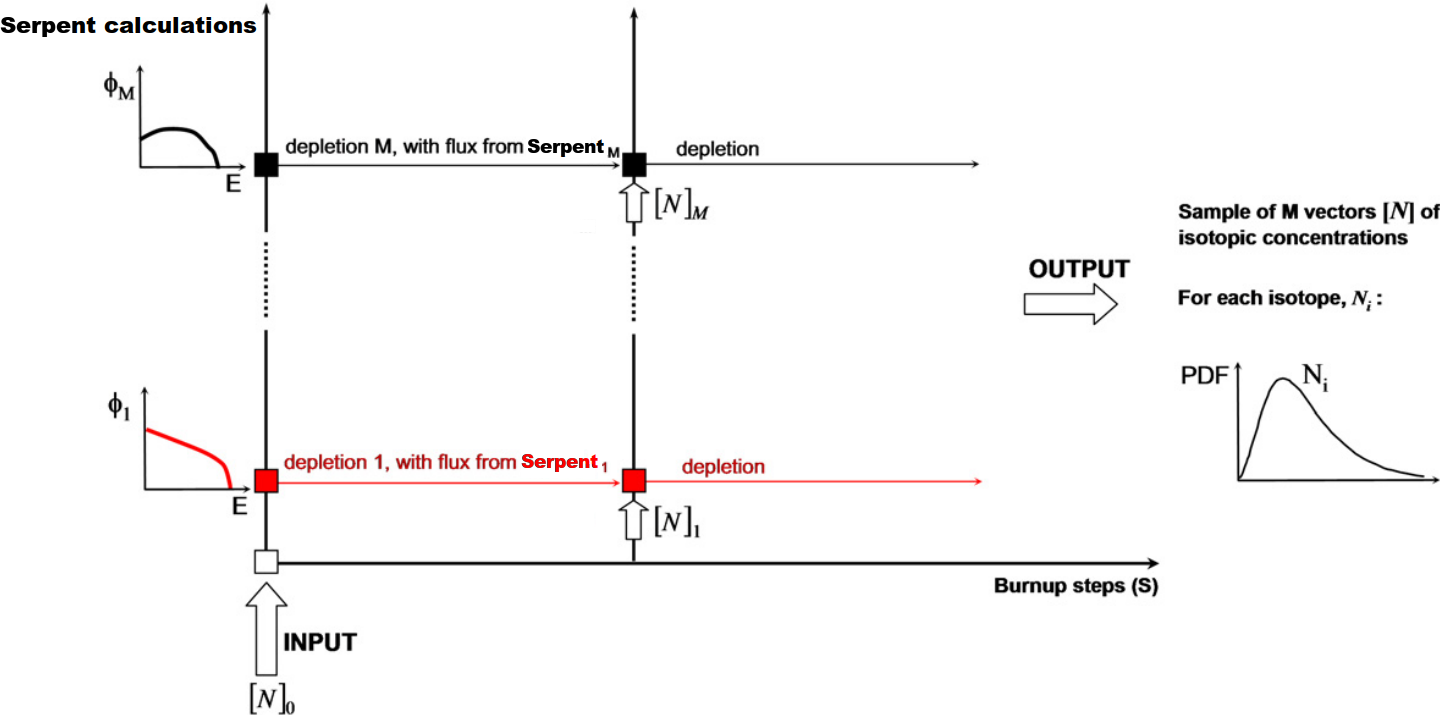
\includegraphics[width=\textwidth]{uq/brute_force_method.png}
	\caption{Methodology of using a normal distribution of random and 
	independent events to estimate uncertainties in final isotopic 
	concentrations (reproduced from Garcia-Herranz \emph{et al.} 
	\cite{garcia-herranz_propagation_2008}). Depletion calculation was 
	performed with the Serpent Monte Carlo code 1000 times by changing only 
	the initial random number.}
	\label{fig:uq-brute-force}
\end{figure}

After running depletion calculations
for all samples, the mean and standard 
deviation of the isotopic concentration can be calculated as
follows
\begin{align}
\overline{N_i} &= \frac{1}{M} \sum_{j=1}^{M} N^{(j)}_i \\
\sigma_{N_i} &= \sqrt{\frac{1}{M-1} \sum_{j=1}^{M} 
(N^{(j)}_i-\overline{N_j})^2}
\intertext{where}
\overline{N_i} &= \mbox{mean concentration of isotope $i$ $[-]$} \nonumber \\
M &= \mbox{number of depletion runs with a unique seed $[-]$} 
\nonumber \\
N^{(j)}_i &= \mbox{concentration of isotope $i$ in the sample $j$ $[-]$.} 
\nonumber
\end{align}

The isotopic concentration $[N]_j$ can then be propagated throughout the 
criticality calculations to estimate the uncertainty of the multiplication 
factor $k_{eff}$. Serpent Monte Carlo code automatically calculates the mean 
and standard deviation of the $k_{eff}$ in each run $j$, which is 
necessary to find the number of runs (samples) required for the convergence of 
$k_{eff}$.

The \gls{TAP} full-core model in Serpent described earlier (see  
Section~\ref{sec:tap-model}) is used for the uncertainty quantification study 
herein. The model benefits from 1/8 symmetry, which allowed me to 
significantly reduce the computational burden without losing accuracy
(Figure~\ref{fig:tap-serpent-plan}). The number of neutron histories was 
selected to compromise between accuracy and computational costs. Running 
15,000 neutrons with 500 active cycles and 200 inactive or “skipped” cycles 
used for source convergence gave a reasonable balance between small 
statistical uncertainty and computation time. Thirty depletion time steps were 
selected for a 30-year depletion simulation (i.e., the isotopic composition is 
stored, and neutron flux is recalculated at the end of each year). 
Additionally, I selected the Chebyshev Rational Approximation Method (CRAM) 
with a predictor-corrector substep \cite{pusa_computing_2010} to reduce 
isotopic 
composition uncertainty. The ENDF/B-VII.1 nuclear data library at 900 K is 
used for all simulations in the current chapter 
\cite{chadwick_endf/b-vii.1_2011}.

\subsection{Results and analysis}
A total of 1000 samples is propagated via the Serpent depletion calculation,  
and the histograms of eigenvalue samples at the \gls{BOL} and \gls{EOL} (30 
\gls{EFPY}) are demonstrated in Figure~\ref{fig:uq-serp-keff-hist}. The 
results show that the effective multiplication factor ($k_{eff}$) mean value 
and the standard deviation due to the stochastic nature of \gls{MC}
both decrease gradually during 30 years of the \gls{TAP} reactor operation. 
An uncertainty in $k_{eff}$ of approximately $35$ $pcm$ is observed at the 
\gls{BOL}, while it slipped to about $29$ $pcm$ at the \gls{EOL}. To obtain 
a set of $M=1000$ vectors of isotopic concentrations in a depletion 
simulation with $S=30$ depletion steps, $M\times S=30,\!000$ Serpent runs were 
performed on Idaho National Laboratory's Falcon cluster. The computational 
time for such an analysis was approximately 1,200 node-hours (4.9 core-years).
\begin{figure}[htp!] % replace 't' with 'b' to 
	\centering
	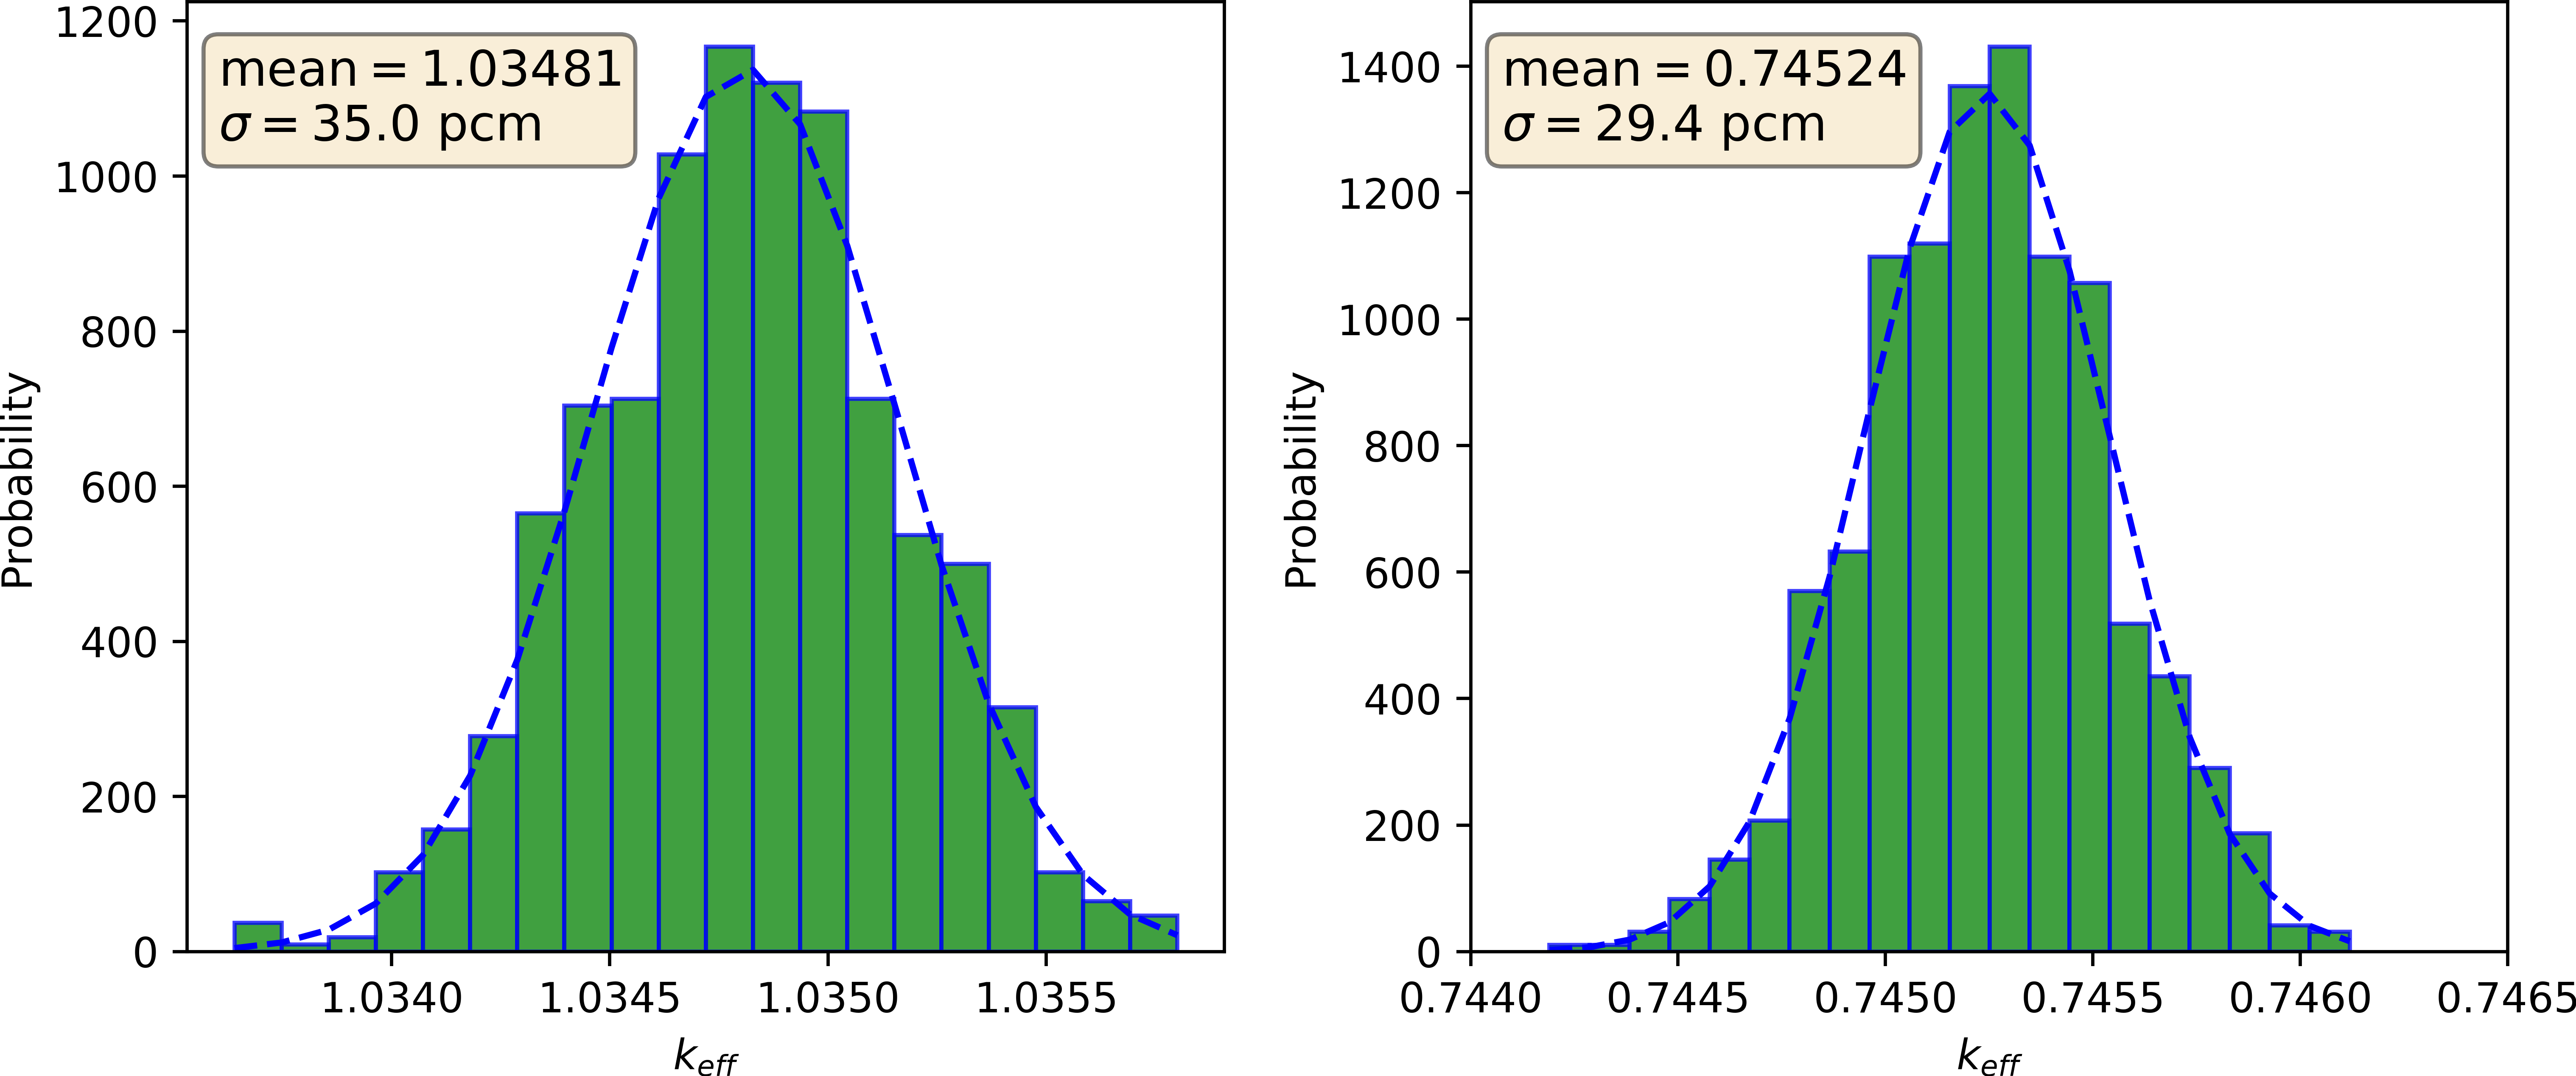
\includegraphics[width=\textwidth]{uq/endf_serpent_keff_hist_for_tap.png}
		\vspace{-4mm}
	\caption{Histograms of $k_{eff}$ samples obtained with 1000 independent 
	Serpent depletion calculations at the \gls{BOL} (left) and \gls{EOL} 
	(right).}
	\label{fig:uq-serp-keff-hist}
\end{figure}

Figure~\ref{fig:uq-serpent-keff-evolution} shows the observed and reported by 
Serpent uncertainties in $k_{eff}$ for the \gls{TAP} core during 30 years of 
operation. Notably, Serpent-calculated uncertainty in the multiplication 
factor is slightly lower than observed uncertainty. This discrepancy is due to 
statistical noise in the output data and agreed with results in the literature 
\cite{wyant_numerical_2012}. Across all 30 depletion steps, the mean observed 
and reported uncertainty in the $k_{eff}$ is $30$ and $25$ $pcm$, 
respectively. A better match in these values could be obtained with more 
samples $M$ (e.g., $M=10,\!000$), which would require substantially more 
computational power.
\begin{figure}[hbp!] % replace 't' with 'b' to 
	\centering
	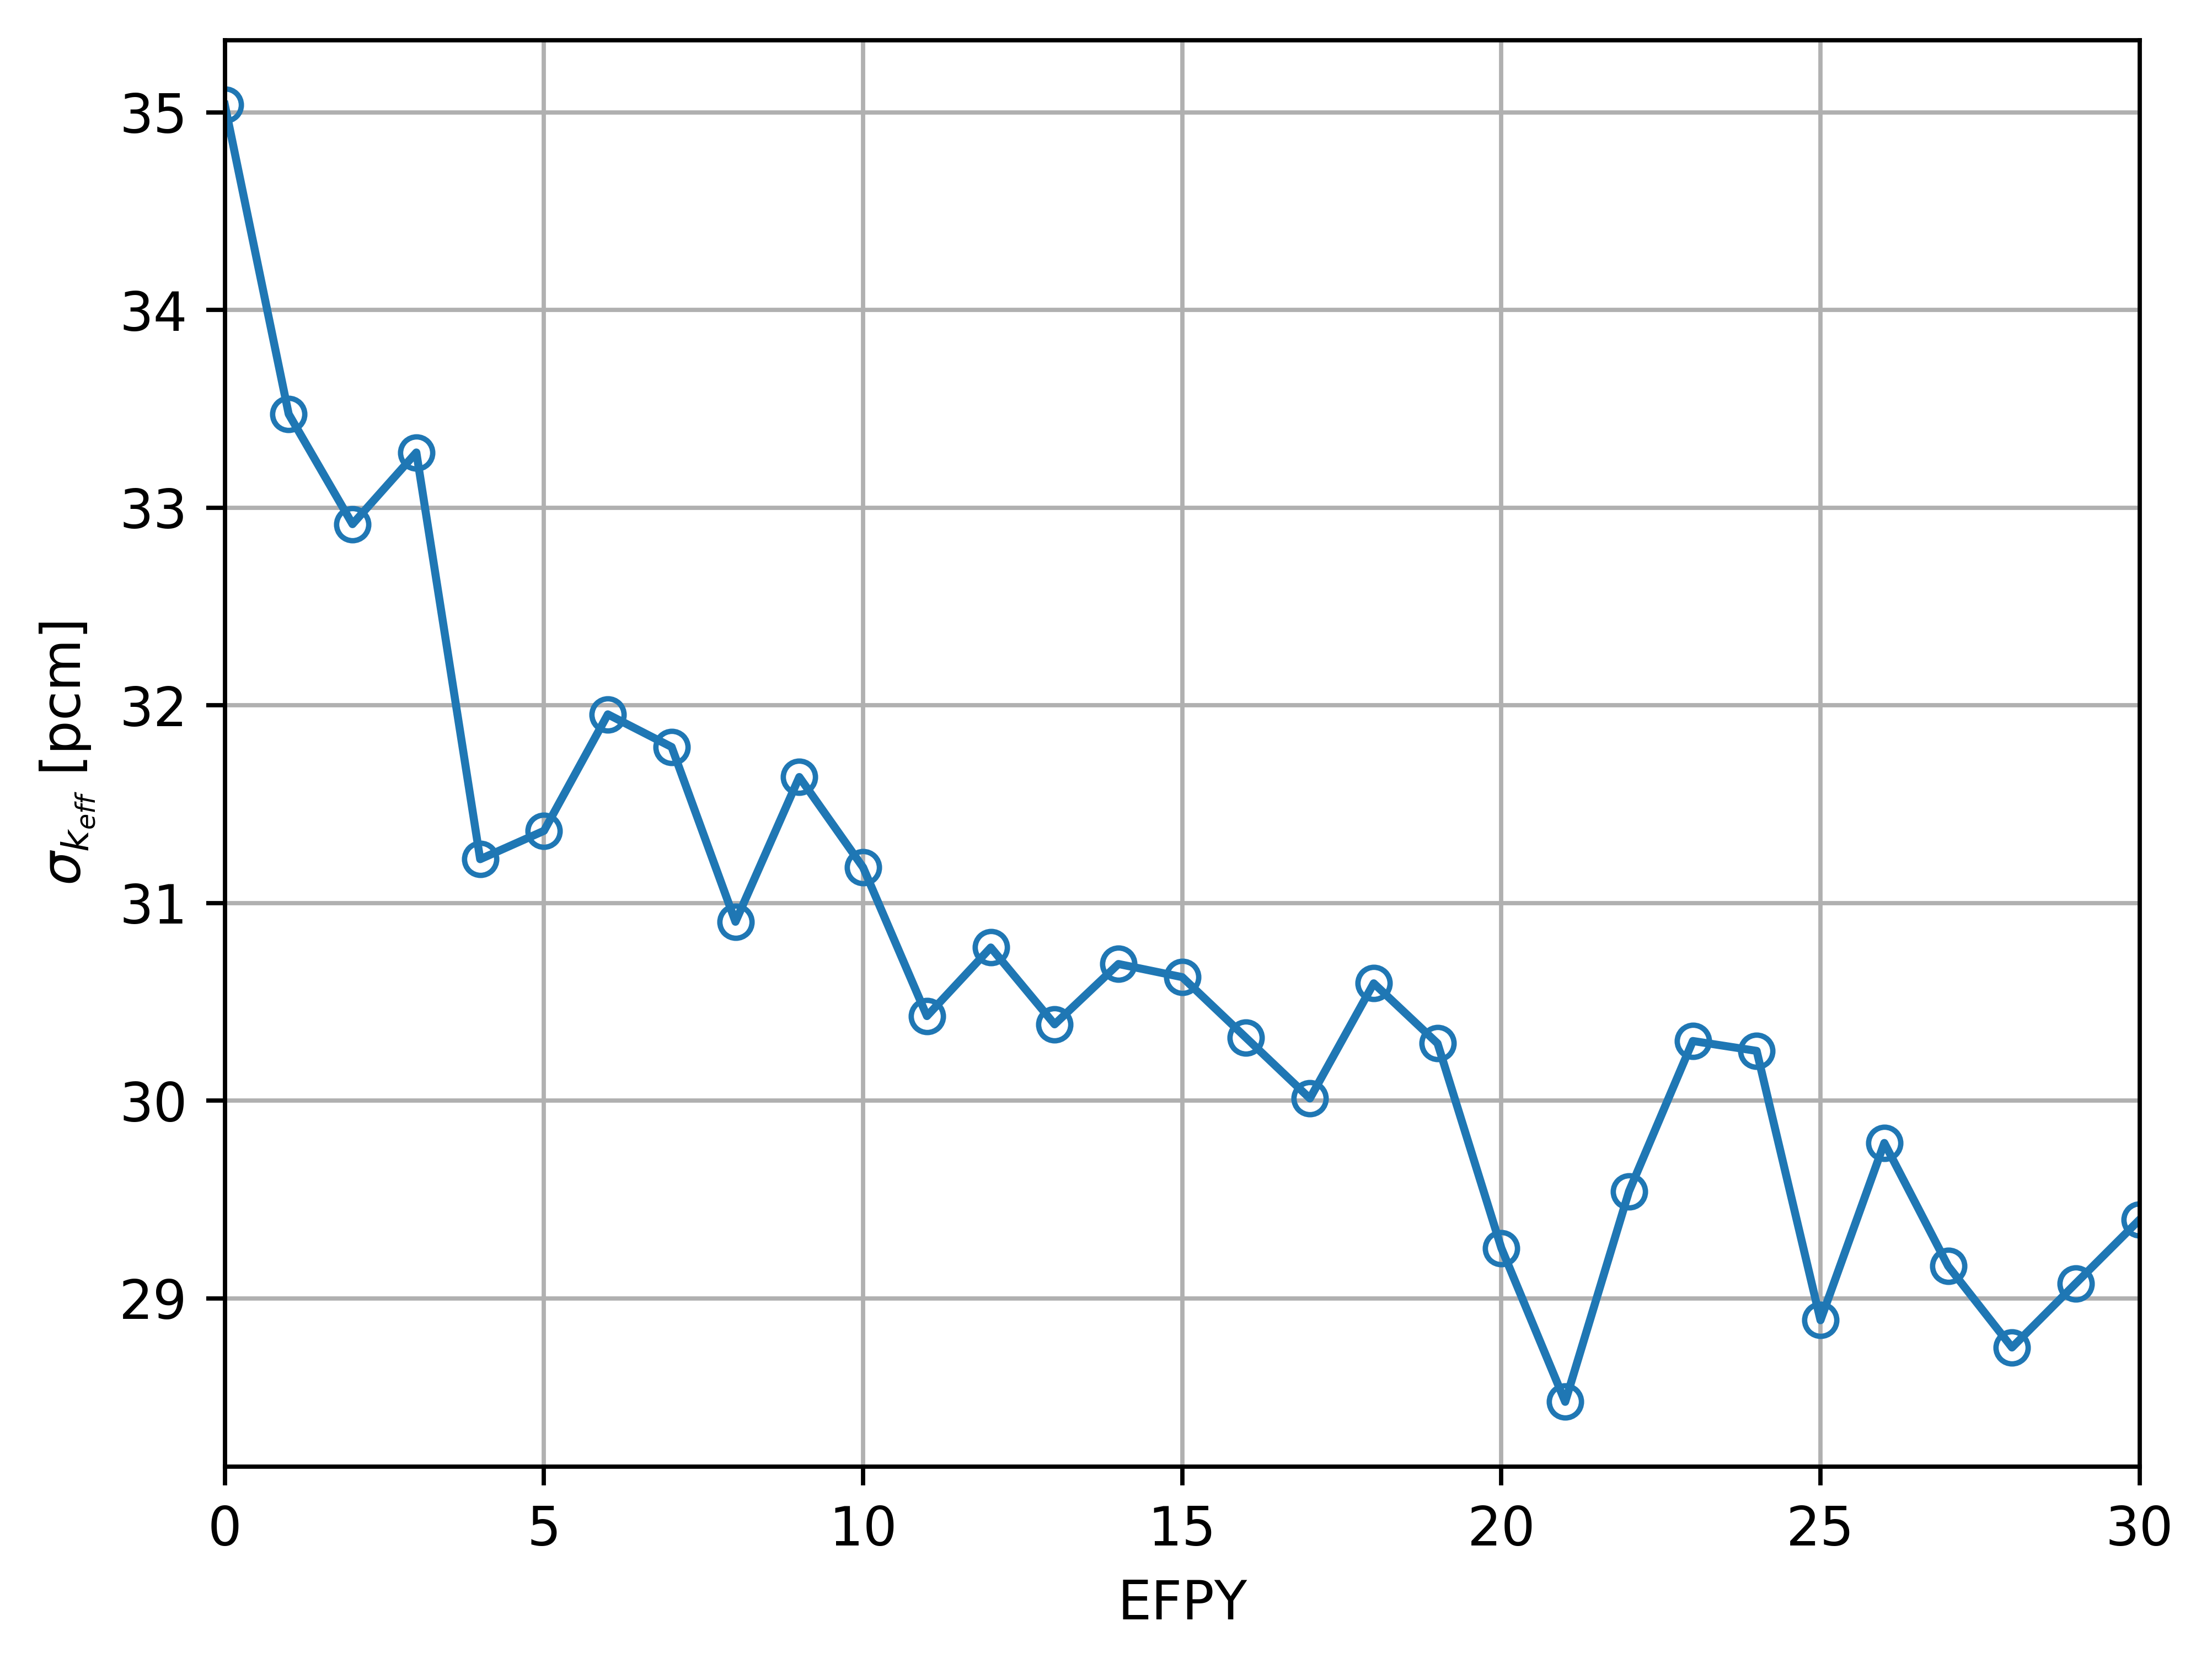
\includegraphics[width=0.83\textwidth]{uq/endf_serpent_keff_dynamics_for_tap.png}
	\caption{Observed and reported by Serpent uncertainty of the effective 
	multiplication factor ($\sigma_{k_{eff}}$) for the full-core \gls{TAP} 
	core model during 30 years of operation.}
	\label{fig:uq-serpent-keff-evolution}
\end{figure}

The current depletion algorithm in Serpent uses the neutron flux solution 
obtained from the \gls{MC} neutron histories to solve the Bateman equations to 
find the isotopic inventory evolution. As was discussed earlier, Serpent 
is unable to estimate the uncertainty of the isotopic number density like it 
does for the $k_{eff}$ (reported $\sigma_{k_{eff}}$ in 
Figure~\ref{fig:uq-serpent-keff-evolution}). Thus, to gain insight into the 
uncertainties in the isotopic inventory, the standard deviation in observed 
isotopic inventories from the 1000 depletion runs was investigated. The 
observed uncertainties for the major actinides and poisonous \glspl{FP} 
resulting from depletion calculations are shown on  
Figures~\ref{fig:uq-serpent-u}, \ref{fig:uq-serpent-pu}, and 
\ref{fig:uq-serpent-xe-i}.

\begin{figure}[htp!] % replace 't' with 'b' to 
	\centering
	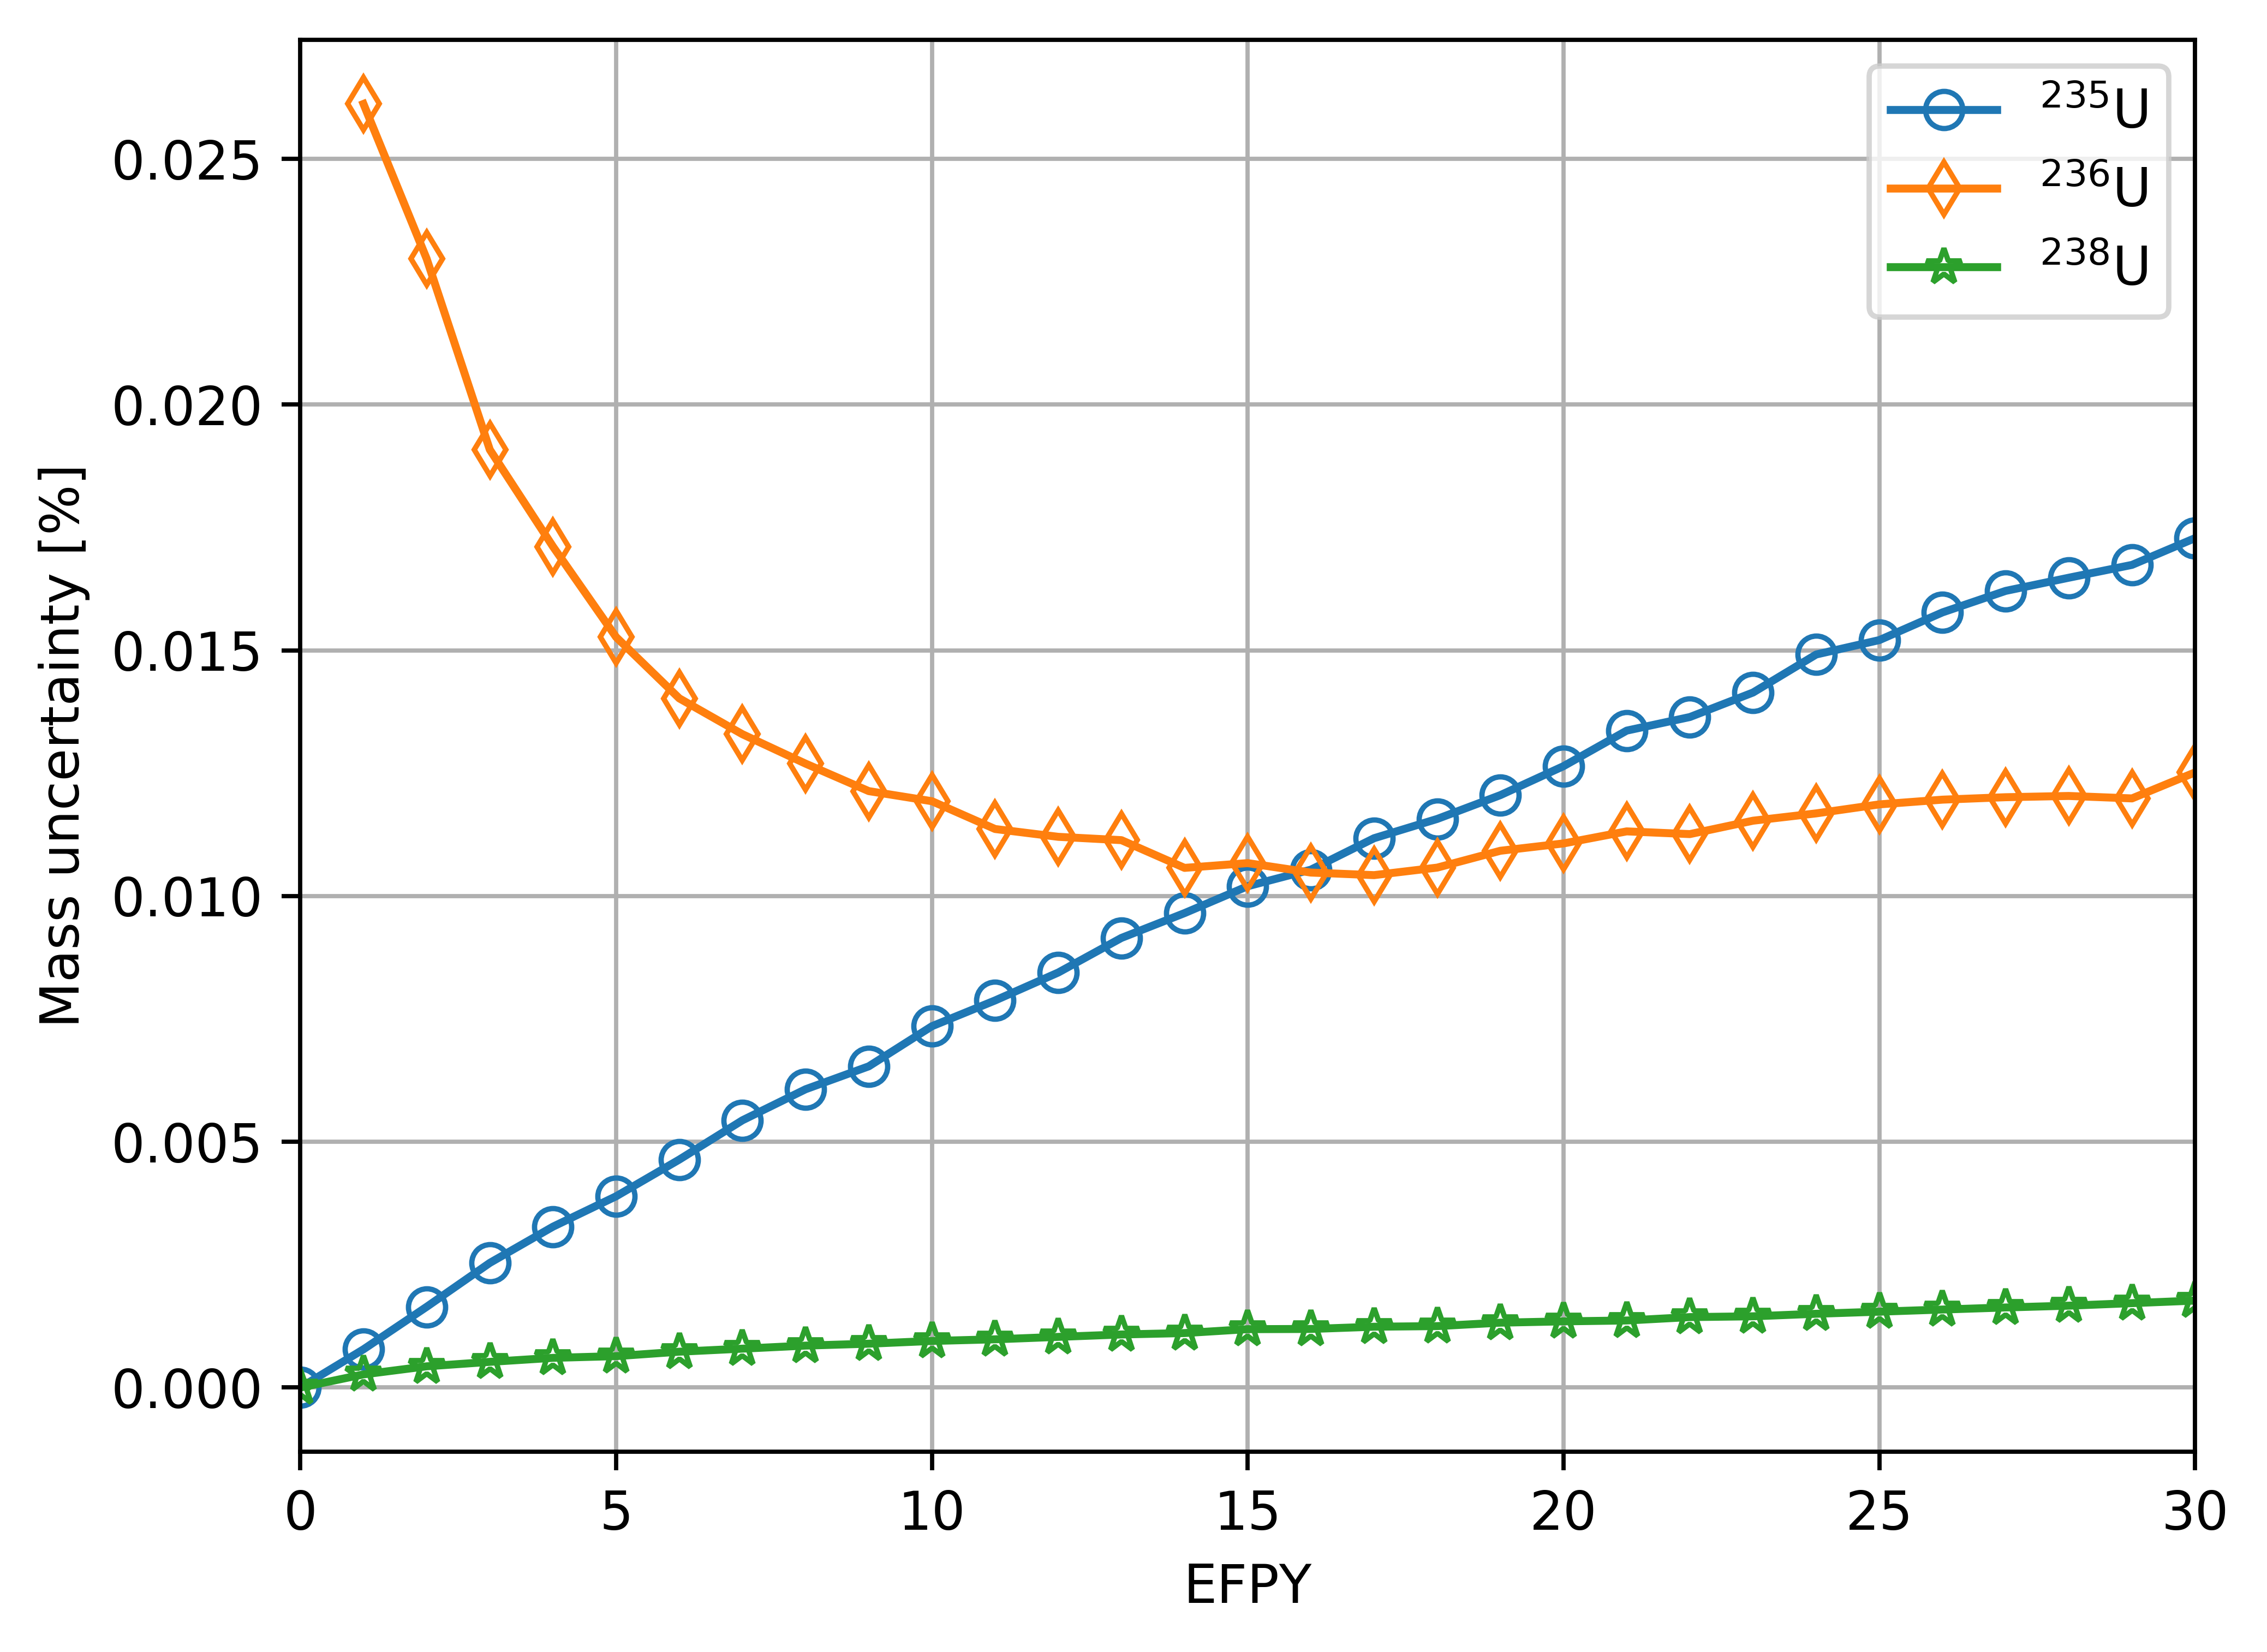
\includegraphics[width=0.8\textwidth]{uq/serpent_mass_std_u.png}
		\vspace{-4mm}
	\caption{Stochastic uncertainty evolution in the uranium isotopic 
	inventory during 30 years of depletion.}
	\label{fig:uq-serpent-u}
\end{figure}

The relative uncertainty of $^{235}$U mass increases with time due to its 
depletion, as the uranium enrichment steadily decreases from 5\% to 0.7\%.
The uncertainty of $^{236}$U mass is 
0.026\% after 30 days of operation when only a few grams of this isotope were 
produced in the core. The uncertainty of $^{236}$U is between 0.011\% and 
0.013\% once the $^{236}$U approaches its equilibrium concentration. The 
relative uncertainties of fissile $^{239}$Pu and $^{241}$Pu are 0.01-0.07\% 
and 0.04-0.18\%, respectively. Mass uncertainties for the 
strongest neutron poison, $^{135}$Xe, and its primary direct precursor, 
$^{135}$I, are 0.0175-0.0275\% and 0.01-0.0175\%, respectively. Overall, 
stochastic error in depletion calculation is larger for isotopes with small 
concentrations in the core due to round-off error. 
Table~\ref{tab:uq-serpent-mean-std-rsd} shows that the stochastic error in the 
isotopic inventories even for an unusually high burnup of 100 MW$_{th}$d/kgU 
(30 EFPY) is negligible ($<0.1$\%).

\begin{figure}[htp!] % replace 't' with 'b' to 
	\centering
	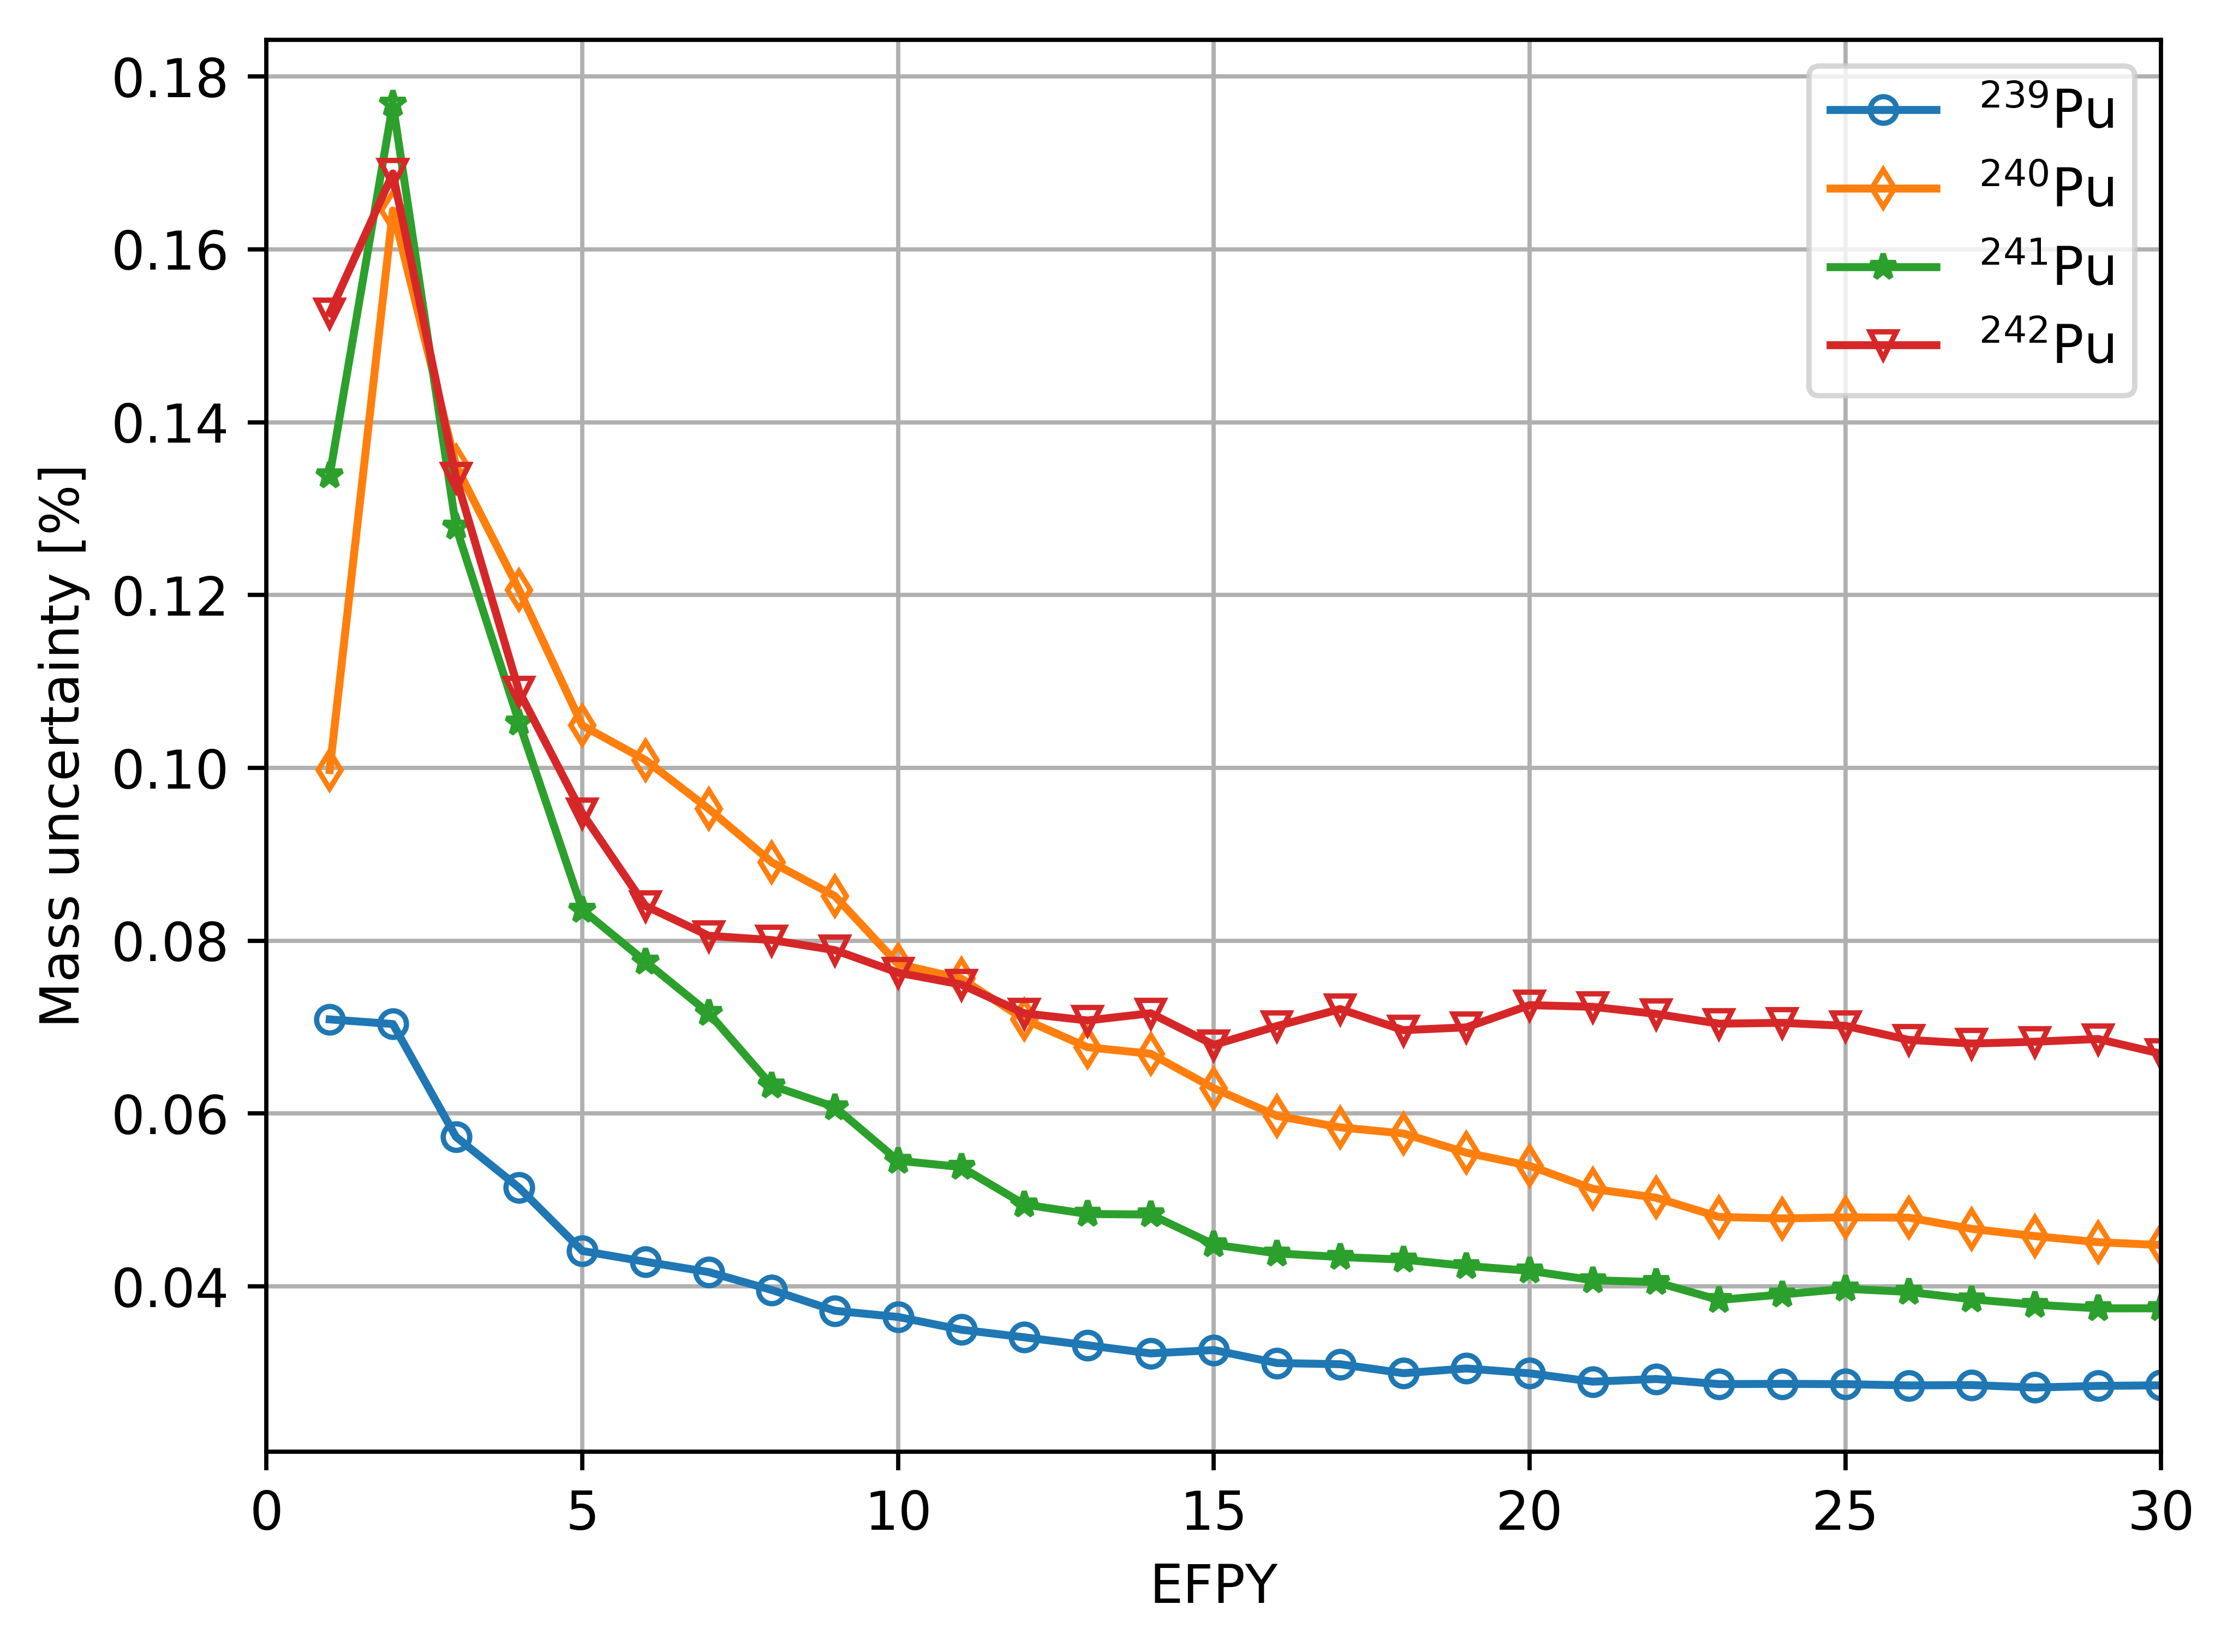
\includegraphics[width=0.73\textwidth]{uq/serpent_mass_std_pu.png}
	\vspace{-3mm}
	\caption{Stochastic uncertainty evolution in the plutonium isotopic 
		inventory during 30 years of depletion.}
	\label{fig:uq-serpent-pu}
\end{figure}
	\vspace{-9mm}
\begin{figure}[hbp!] % replace 't' with 'b' to 
	\centering
	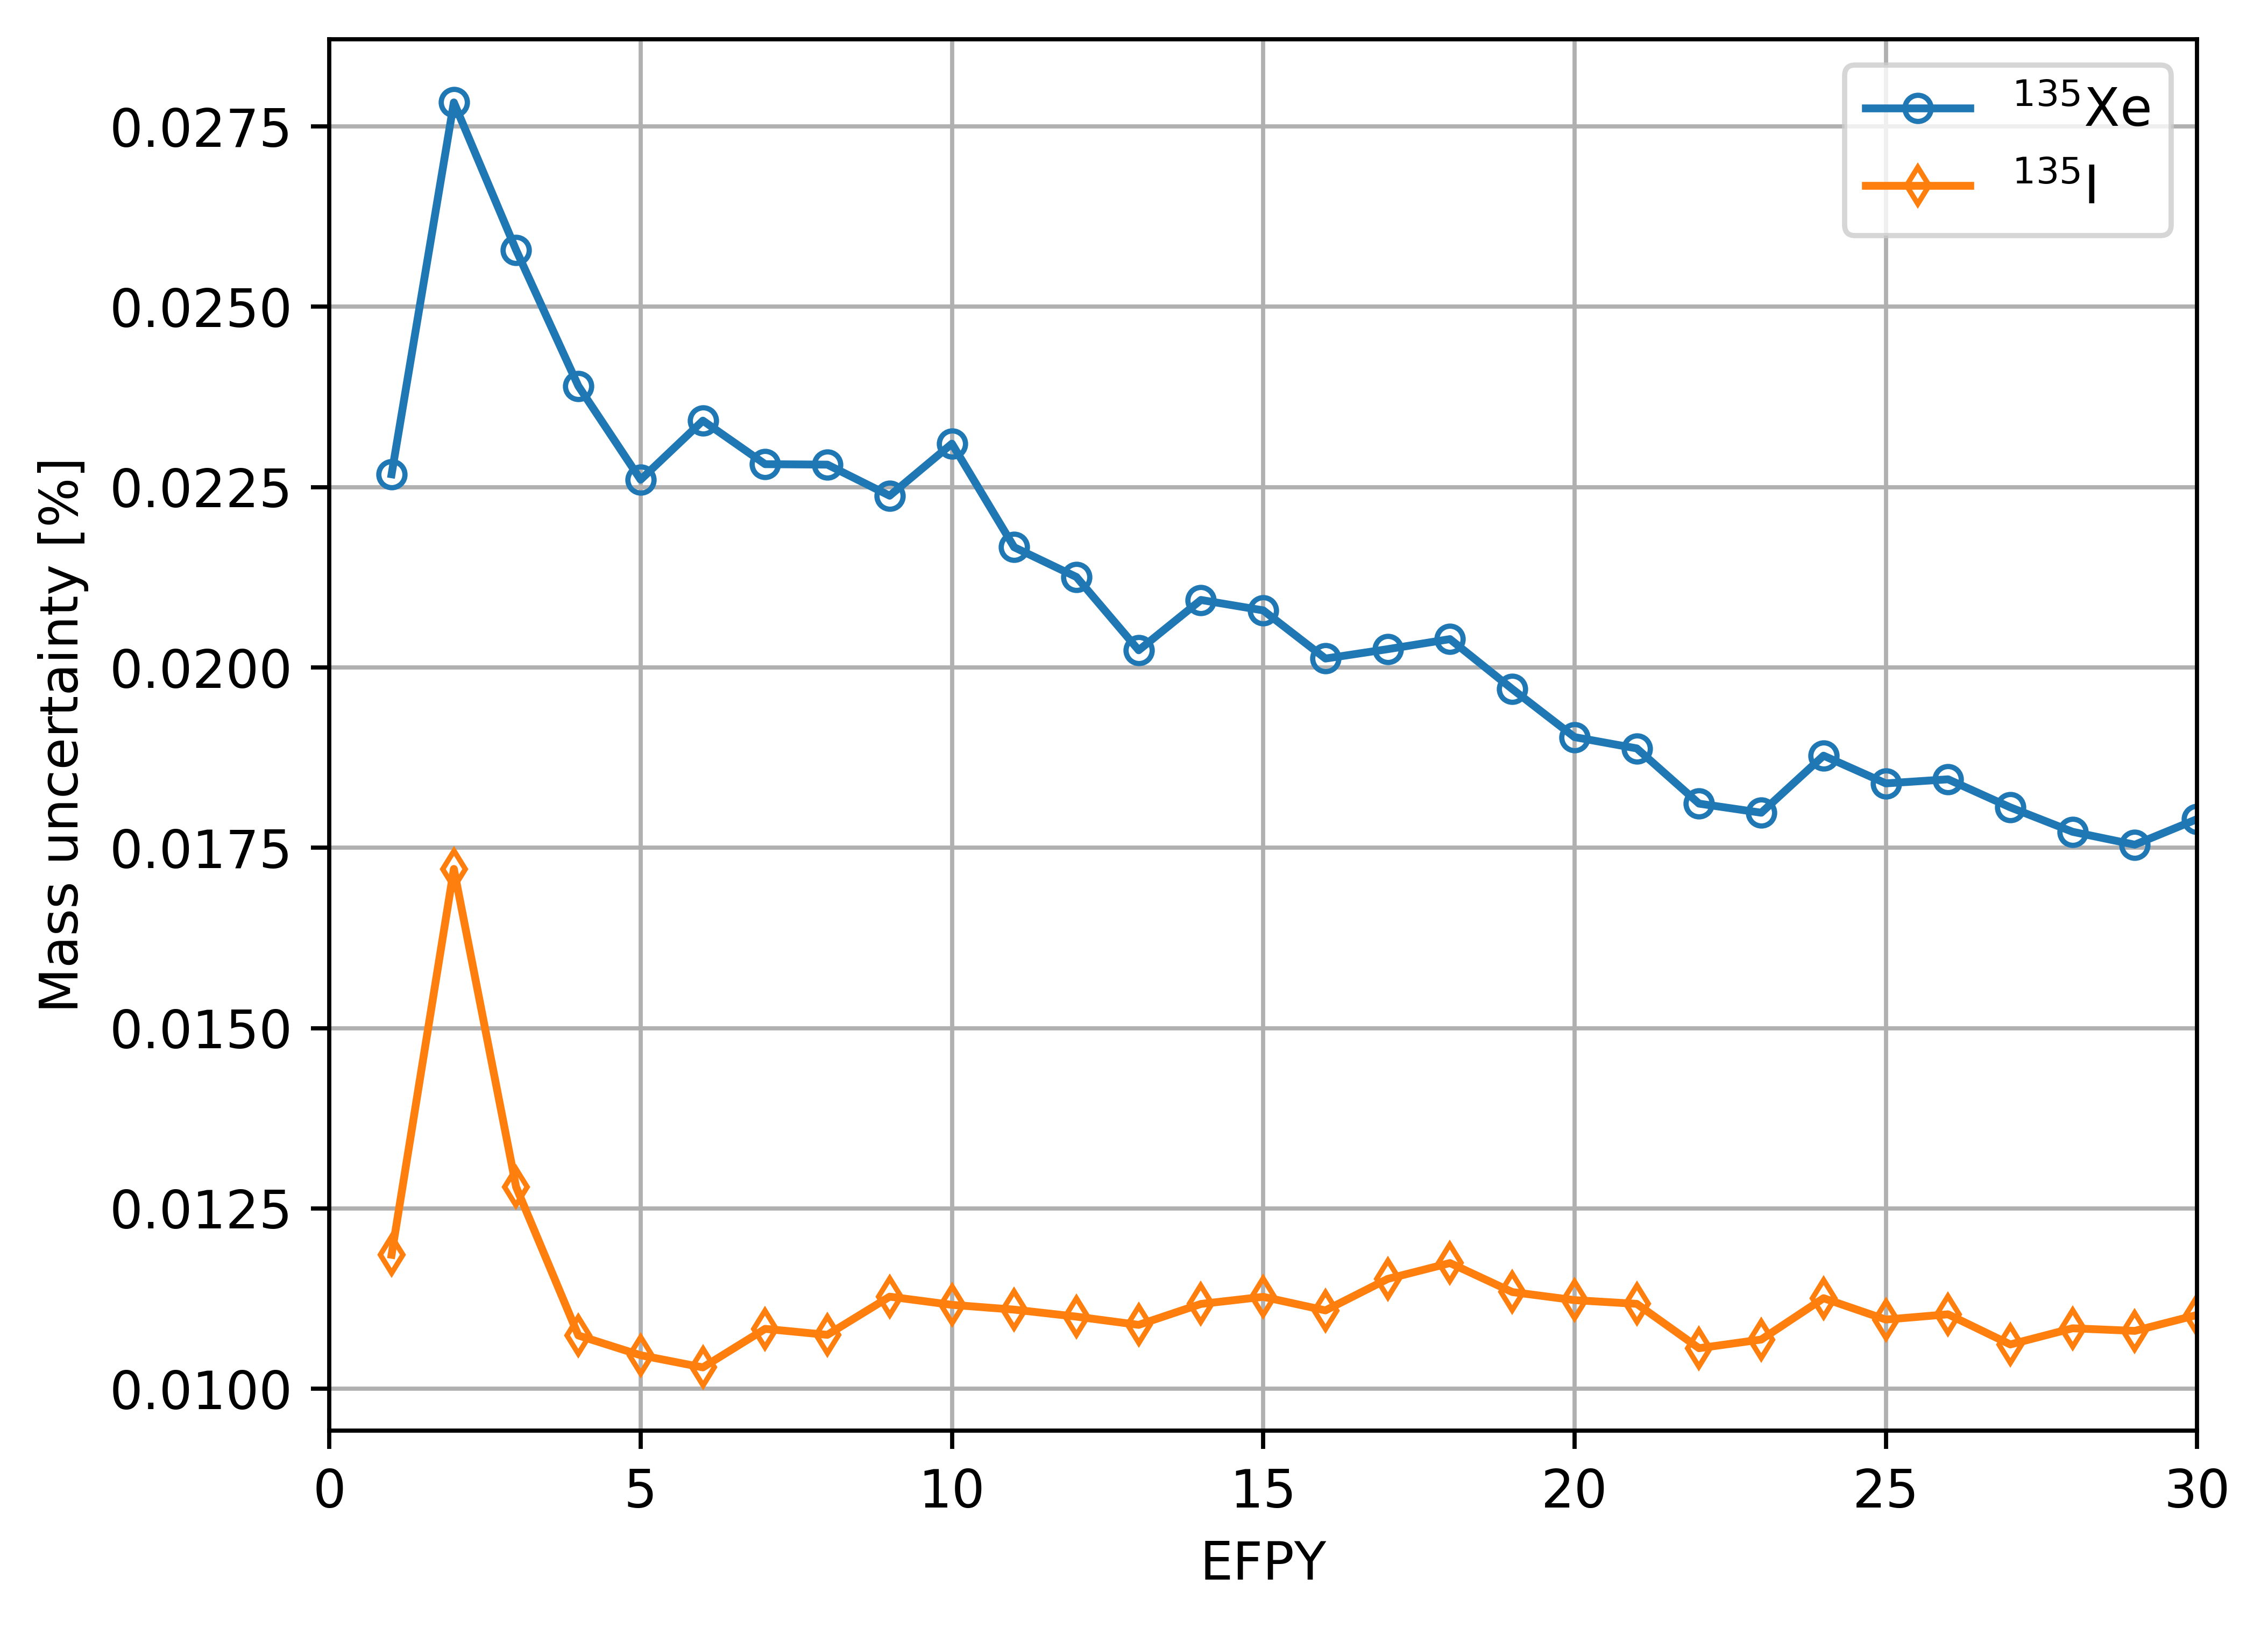
\includegraphics[width=0.73\textwidth]{uq/serpent_mass_std_xe_i.png}
		\vspace{-3mm}
	\caption{Stochastic uncertainty evolution in $^{135}$Xe and $^{135}$I 
	isotopic inventory during 30 years of depletion.}
	\label{fig:uq-serpent-xe-i}
\end{figure}


%%%%%%%%%%%%%%%%%%%%%%%%%%%%%%%%%%%%%%%%
\begin{table}[htp!]
	\centering
	\caption{Mean value, Standard Deviation (STD), and Relative Standard 
	Deviation (RSD) of mass for the major isotopes after 30-year depletion 
	analysis for the \gls{TAP} reactor. Only the stochastic error in the Monte 
	Carlo calculations is considered.}
	\begin{tabularx}{0.7\textwidth}{L R R R R}
		\hline
		\textbf{Isotope}  & \textbf{Mean [kg]} & \textbf{STD [kg]} & 
		\textbf{RSD [\%]}\\ \hline
		$^{234}$U  & 25.8  & 0.0075 & .0290\% \\
		$^{235}$U  & 789.9 & 0.1365 & .0173\% \\
		$^{236}$U  & 1149.5& 0.1439 & .0125\% \\
		$^{238}$U  & 112,084.8 & 1.9835 & .0018\% \\
		$^{238}$Pu & 405.5 & 0.0884 & .0218\% \\
		$^{239}$Pu & 5554.3& 1.5860 & .0286\% \\
		$^{240}$Pu & 1230.2& 0.5510 & .0448\% \\
		$^{241}$Pu & 763.1 & 0.2859 & .0375\% \\
		$^{242}$Pu & 139.0 & 0.0930  & .0669\% \\
		$^{241}$Am & 218.3 & 0.0566  & .0259\% \\
		$^{135}$Xe & 0.03  & $<0.0001$& .0179\% \\
		$^{135}$I  & 0.02  & $<0.0001$& .0110\% \\ \hline
	\end{tabularx}
	\label{tab:uq-serpent-mean-std-rsd}
	\vspace{-0.9em}
\end{table}
%%%%%%%%%%%%%%%%%%%%%%%%%%%%%%%%%%%%%%%%%%%%%%%%%%%%%%%%%%%%%%%%%%%%%%%%%%%%%%%

All results presented in Figures~\ref{fig:uq-serpent-u}, 
\ref{fig:uq-serpent-pu}, \ref{fig:uq-serpent-xe-i} and  
Table~\ref{tab:uq-serpent-mean-std-rsd} are based on 1000 samples (e.g., 1000 
independent Serpent depletion simulations with unique seed values for the 
random number sequence). Figure~\ref{fig:uq-serpent-convergence} shows the 
convergence of $k_{eff}$ and $^{235}$U mass uncertainty with the number of 
samples. Notably, 300 samples were enough for $\sigma_{k_{eff}}$ convergence. 
The $^{235}$U mass uncertainty at the \gls{EOL} decreases steadily 
with the number of samples, but even 400 samples are sufficient to obtain 
reasonable uncertainty ($<0.02$\%). 
Finally, it is possible to reduce the stochastic uncertainty in the isotopic 
inventory to almost zero by substantially increasing the neutron population 
(number of neutron histories and active cycles); however, it is extremely 
inefficient because Monte Carlo converges sublinearly ($O(\sqrt{N})$).
\begin{figure}[htp!] % replace 't' with 'b' to 
	\centering
	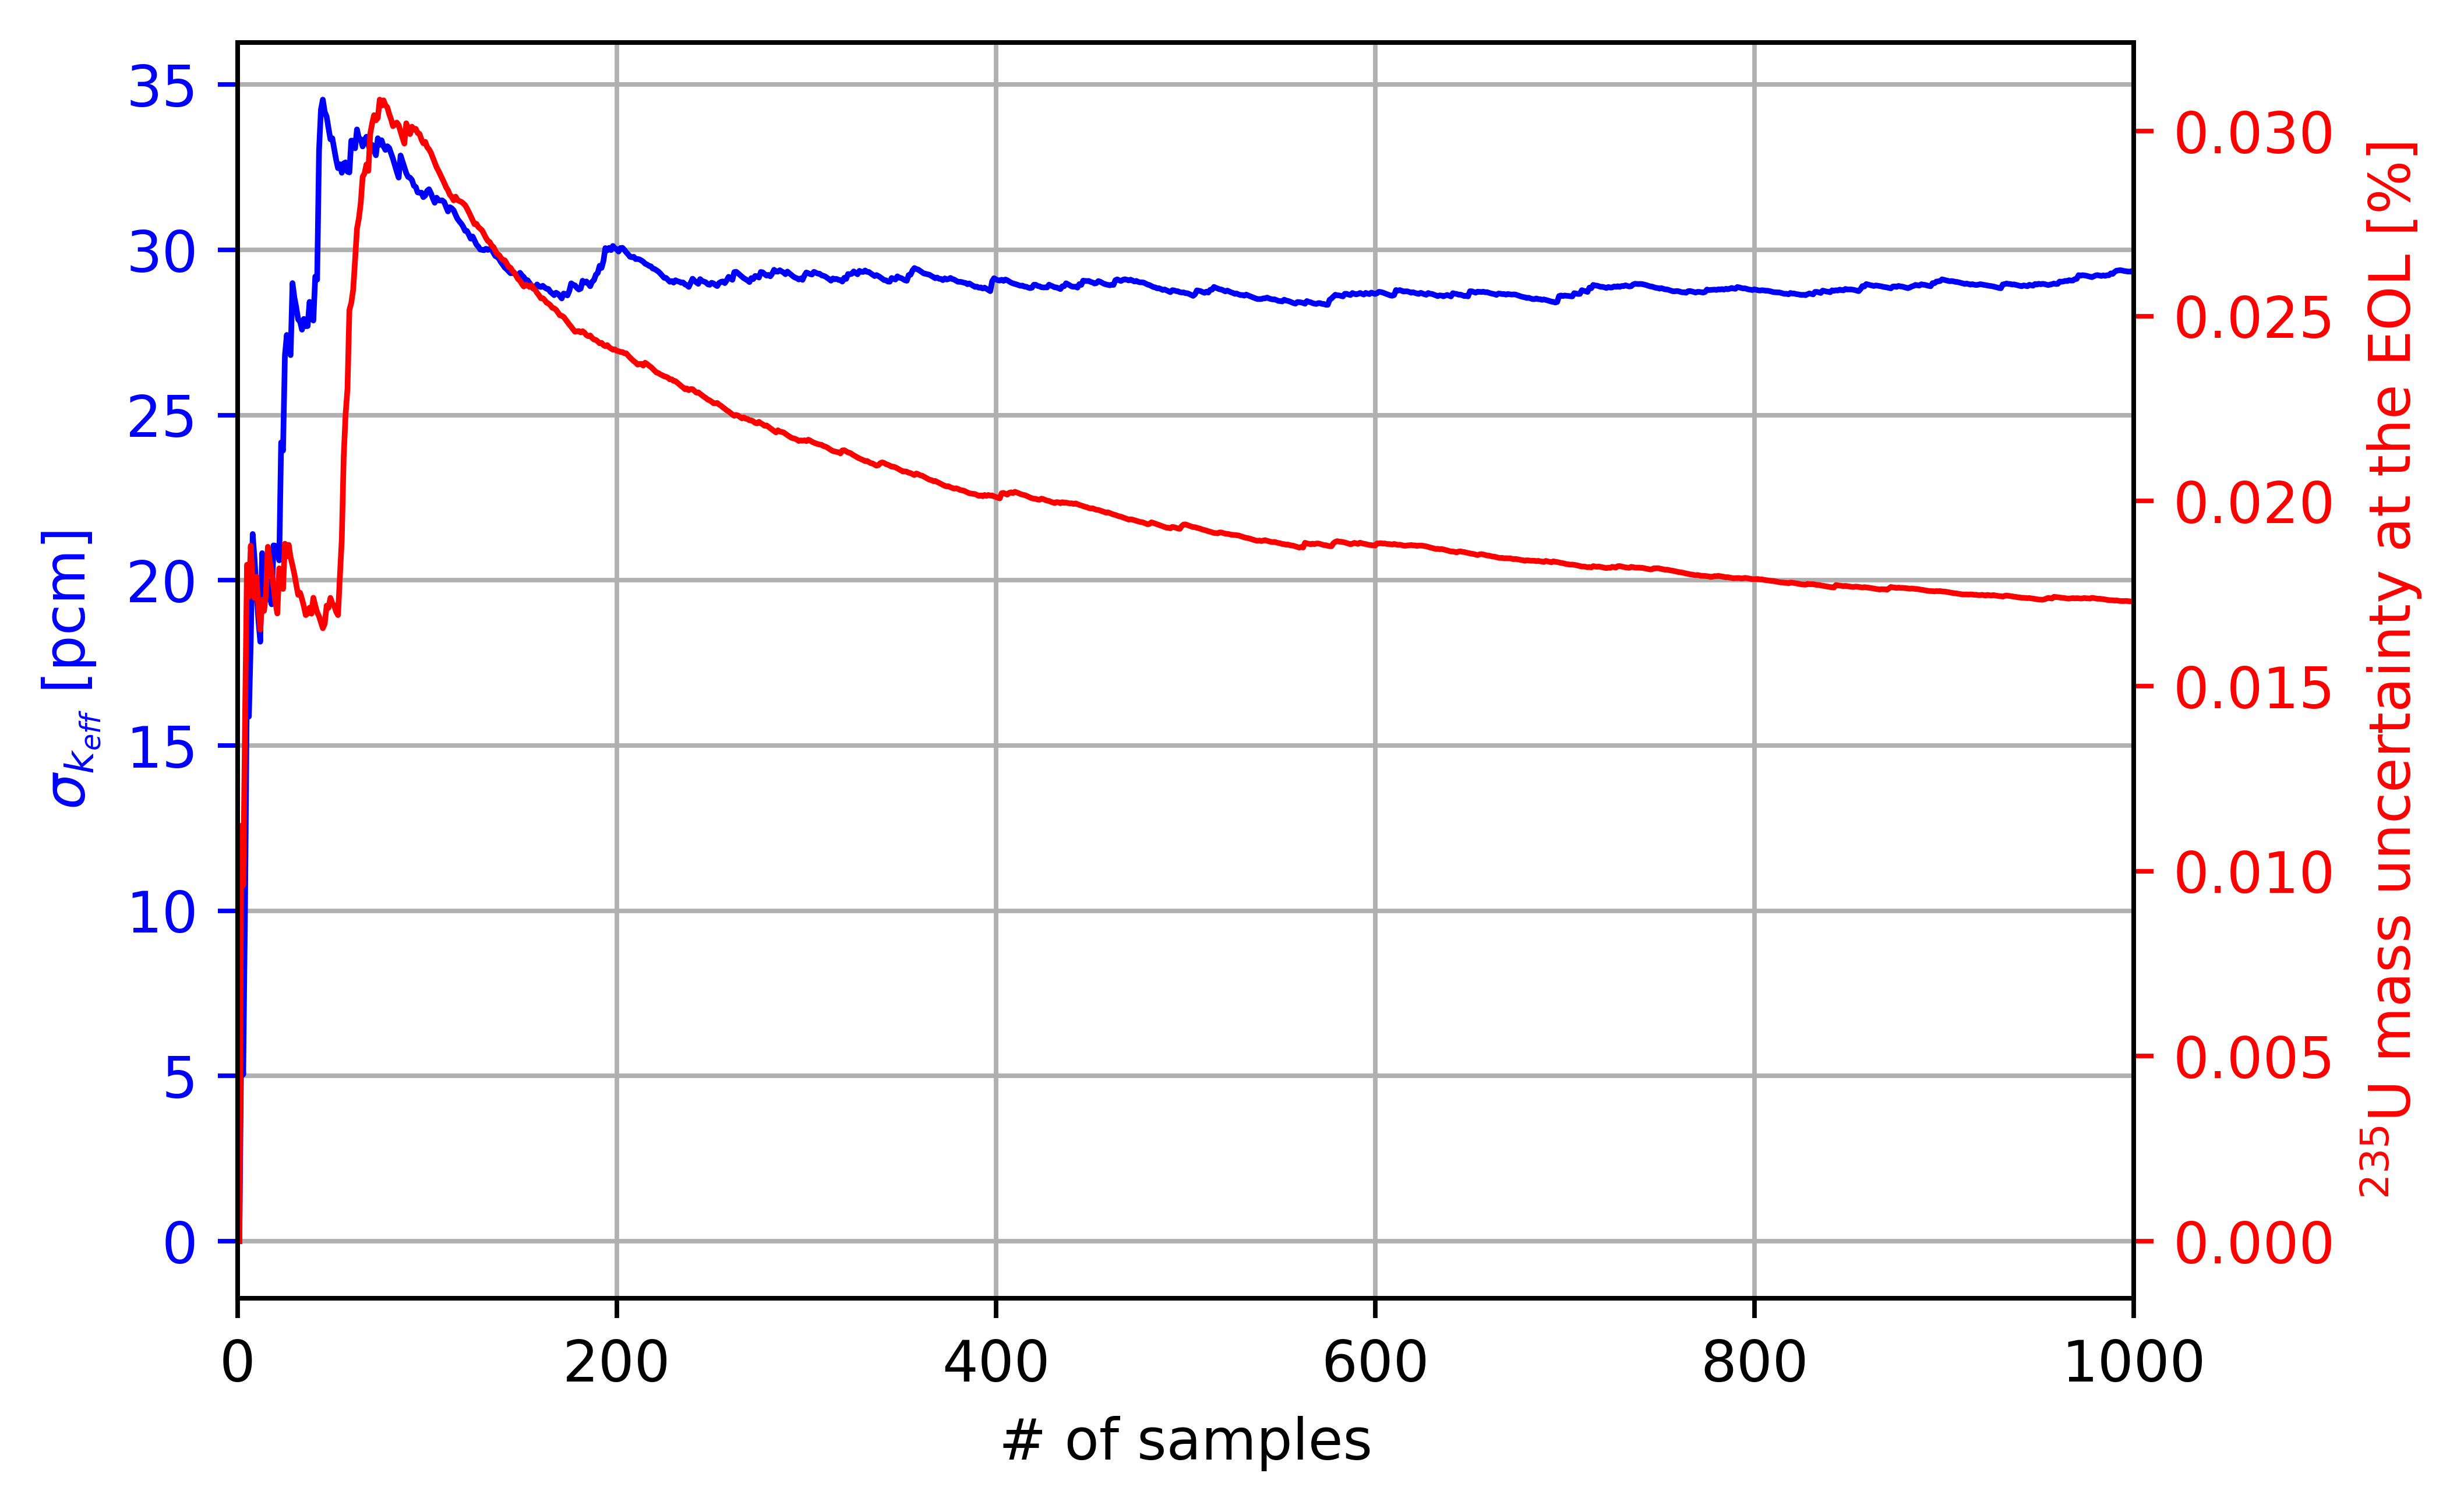
\includegraphics[width=\textwidth]{uq/serpent_convergance_for_tap.png}
	\caption{Convergence of $k_{eff}$ and $^{235}$U mass uncertainties due to 
	the statistical error in Monte Carlo as a function of samples number.}
	\label{fig:uq-serpent-convergence}
\end{figure}
\FloatBarrier


\section{Nuclear data-related uncertainty in the isotopic inventory}
This section focuses on evaluating uncertainty in a depletion calculation 
caused by uncertainties in nuclear data, namely, cross sections, fission 
yields, and decay constants. I used deterministic $S_N$ code SCALE/TRITON 
\cite{rearden_scale_2018} to avoid statistical errors, which are inevitable 
when using any Monte Carlo transport software (e.g., Serpent), to estimate 
only nuclear data-related uncertainty.

\subsection{Methodology of uncertainty propagation by a random sampling}
The nuclear data uncertainties are propagated through fuel depletion 
calculation using a random sampling method\footnote{Sometimes researchers also 
called it ``Monte Carlo sampling," \cite{radaideh_using_2019-1} ``brute 
force method,"\cite{garcia-herranz_propagation_2008} or ``Fast Total Monte 
Carlo" \cite{rochman_nuclear_2014}. However, in this chapter, this method is 
called ``random  sampling."}. The multi-step sequence of deterministic 
neutronics and isotopic transmutation could be regarded as a single 
process with input parameters (cross sections, fission yields, decay 
constants) and an output (isotopic inventory). This sequence runs a 
large number of times, each time using a different nuclear data file (sample). 
This collection of random nuclear data files is produced by the SCALE Sampler 
module from a multivariate normal distribution using covariance matrices in 
the 56-group covariance library \cite{rearden_scale_2018, 
radaideh_novel_2019-1}. This approach is summarized in the flowchart 
(Figure~\ref{fig:uq-sampler}).

After generating the collection of random nuclear data files, the depletion 
calculations are performed for each sample with SCALE. This work uses NEWT, a
2D-deterministic transport code, coupled with ORIGEN. ORIGEN solves a set of 
the Bateman equations using NEWT-calculated neutron fluxes. The unit cell 
model is used to achieve reasonable computing costs while providing an 
accurate neutron spectrum for depletion calculations 
(Figure~\ref{fig:uq-tap-pincell}) \cite{betzler_molten_2017, 
rykhlevskii_fuel_2019, betzler_modeling_2020}. For this unit cell model, an 
8$\times$8 mesh with the reflective boundary condition is used. The 56-group 
ENDF/B-VII.1 nuclear data library along with the 56-group covariance library 
are 
used in depletion calculations. The full-core 3-D depletion 
calculation can be performed if NEWT is replaced with KENO-VI, which 
is a three-dimensional Monte Carlo neutron transport code, that might be 
coupled with ORIGEN for performing depletion calculations. However, two 
reasons make it impractical because: 
(1) it requires enormous computing cost, (2) it introduces stochastic error 
due to the statistical nature of the \gls{MC} method, and 
(3) it cannot be applied to continuous energy Monte Carlo calculations 
\cite{rearden_scale_2018}.
\begin{figure}[htp!] % replace 't' with 'b' to 
	\centering
	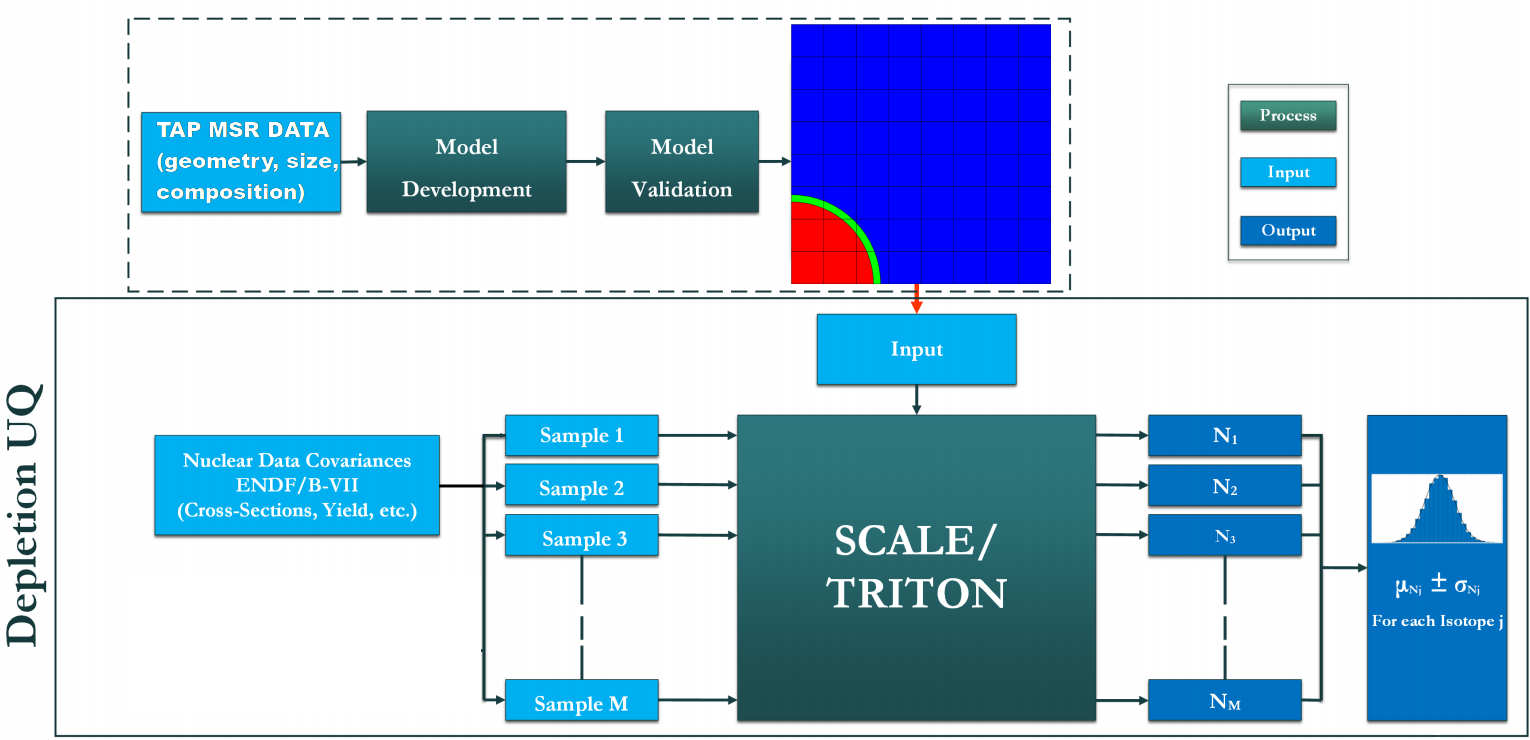
\includegraphics[width=\textwidth]{uq/majdi_scale_scheme.png}
	\caption{Flowchart of the depletion uncertainty quantification 
		using SCALE Sampler (figure courtesy of Majdi I. Radaideh 
		\cite{radaideh_novel_2019-1}).}
	\label{fig:uq-sampler}
\end{figure}
	\vspace{-7mm}
\begin{figure}[hbp!] % replace 't' with 'b' to 
	\centering
	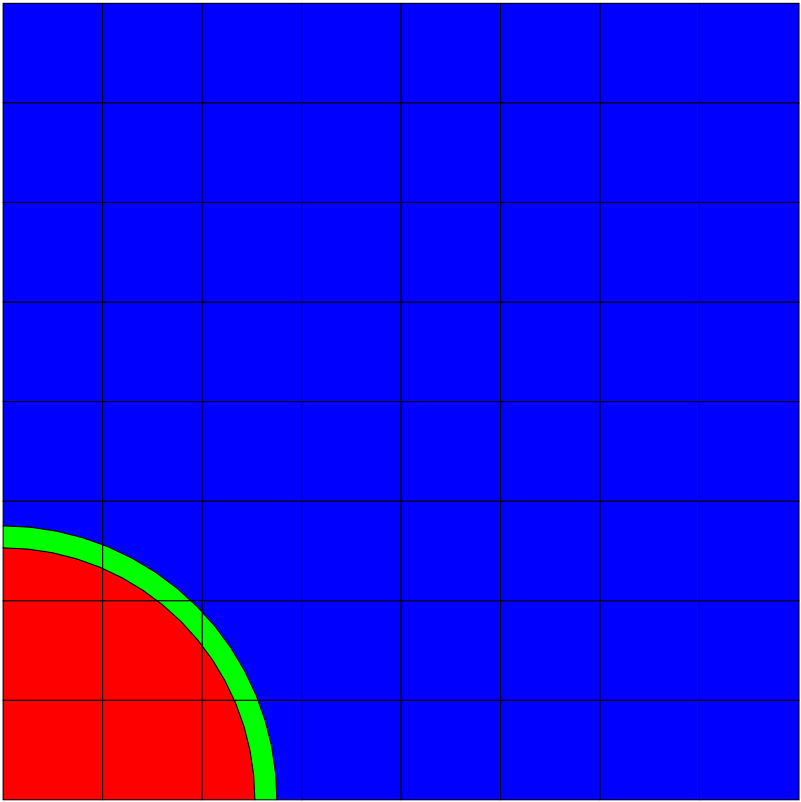
\includegraphics[width=0.36\textwidth]{uq/tap_pin_for_scale.png}
	\caption{Unit cell model representation for the \gls{TAP} \gls{MSR} in 
	SCALE.}
	\label{fig:uq-tap-pincell}
\end{figure}

The fuel salt composition, total depletion time, depletion time steps, and 
power density match the ones given in Section~\ref{sec:uq-stochastic} for 
consistency of comparison. Overall, I repeated 800 SCALE depletion 
calculations using perturbed cross sections, fission yields, and decay 
constants, assuming that the probability density functions are multivariate 
normal distributions with covariances provided with the SCALE nuclear data 
library.


\subsection{Results and analysis}
Figure~\ref{fig:uq-scale-kinf-hist} shows the histograms of samples for the 
infinite multiplication factor ($k_{\infty}$) at the \gls{BOL} and \gls{EOL} 
(30 \gls{EFPY}) for 800 total random samples. Similar to stochastic 
uncertainty, the results show that the $k_{\infty}$ standard deviation due to 
the nuclear data uncertainty decreases during 30 years of the \gls{TAP} 
reactor operation. An uncertainty of about 804 $pcm$ in $k_{\infty}$ is 
observed at startup, while it is reduced to 469 $pcm$ at the \gls{EOL}. 
Notably, nuclear data-related uncertainty in the multiplication factor is 
about 20 times larger than uncertainty due to the stochastic error (see 
Section~\ref{sec:uq-stochastic}), which agrees well with results in the 
literature \cite{takeda_estimation_1999, garcia-herranz_propagation_2008}. 
Thanks to the unit cell model and a fast deterministic $S_N$ NEWT transport 
code, the computational time for producing 800 random samples was only 576 
core-days. Generation of the 800 samples with better accuracy (full-core, 
three-dimensional model solved with KENO-VI) would require substantially more 
computational power (about 10,000 times more).
\begin{figure}[htp!] % replace 't' with 'b' to 
	\centering
	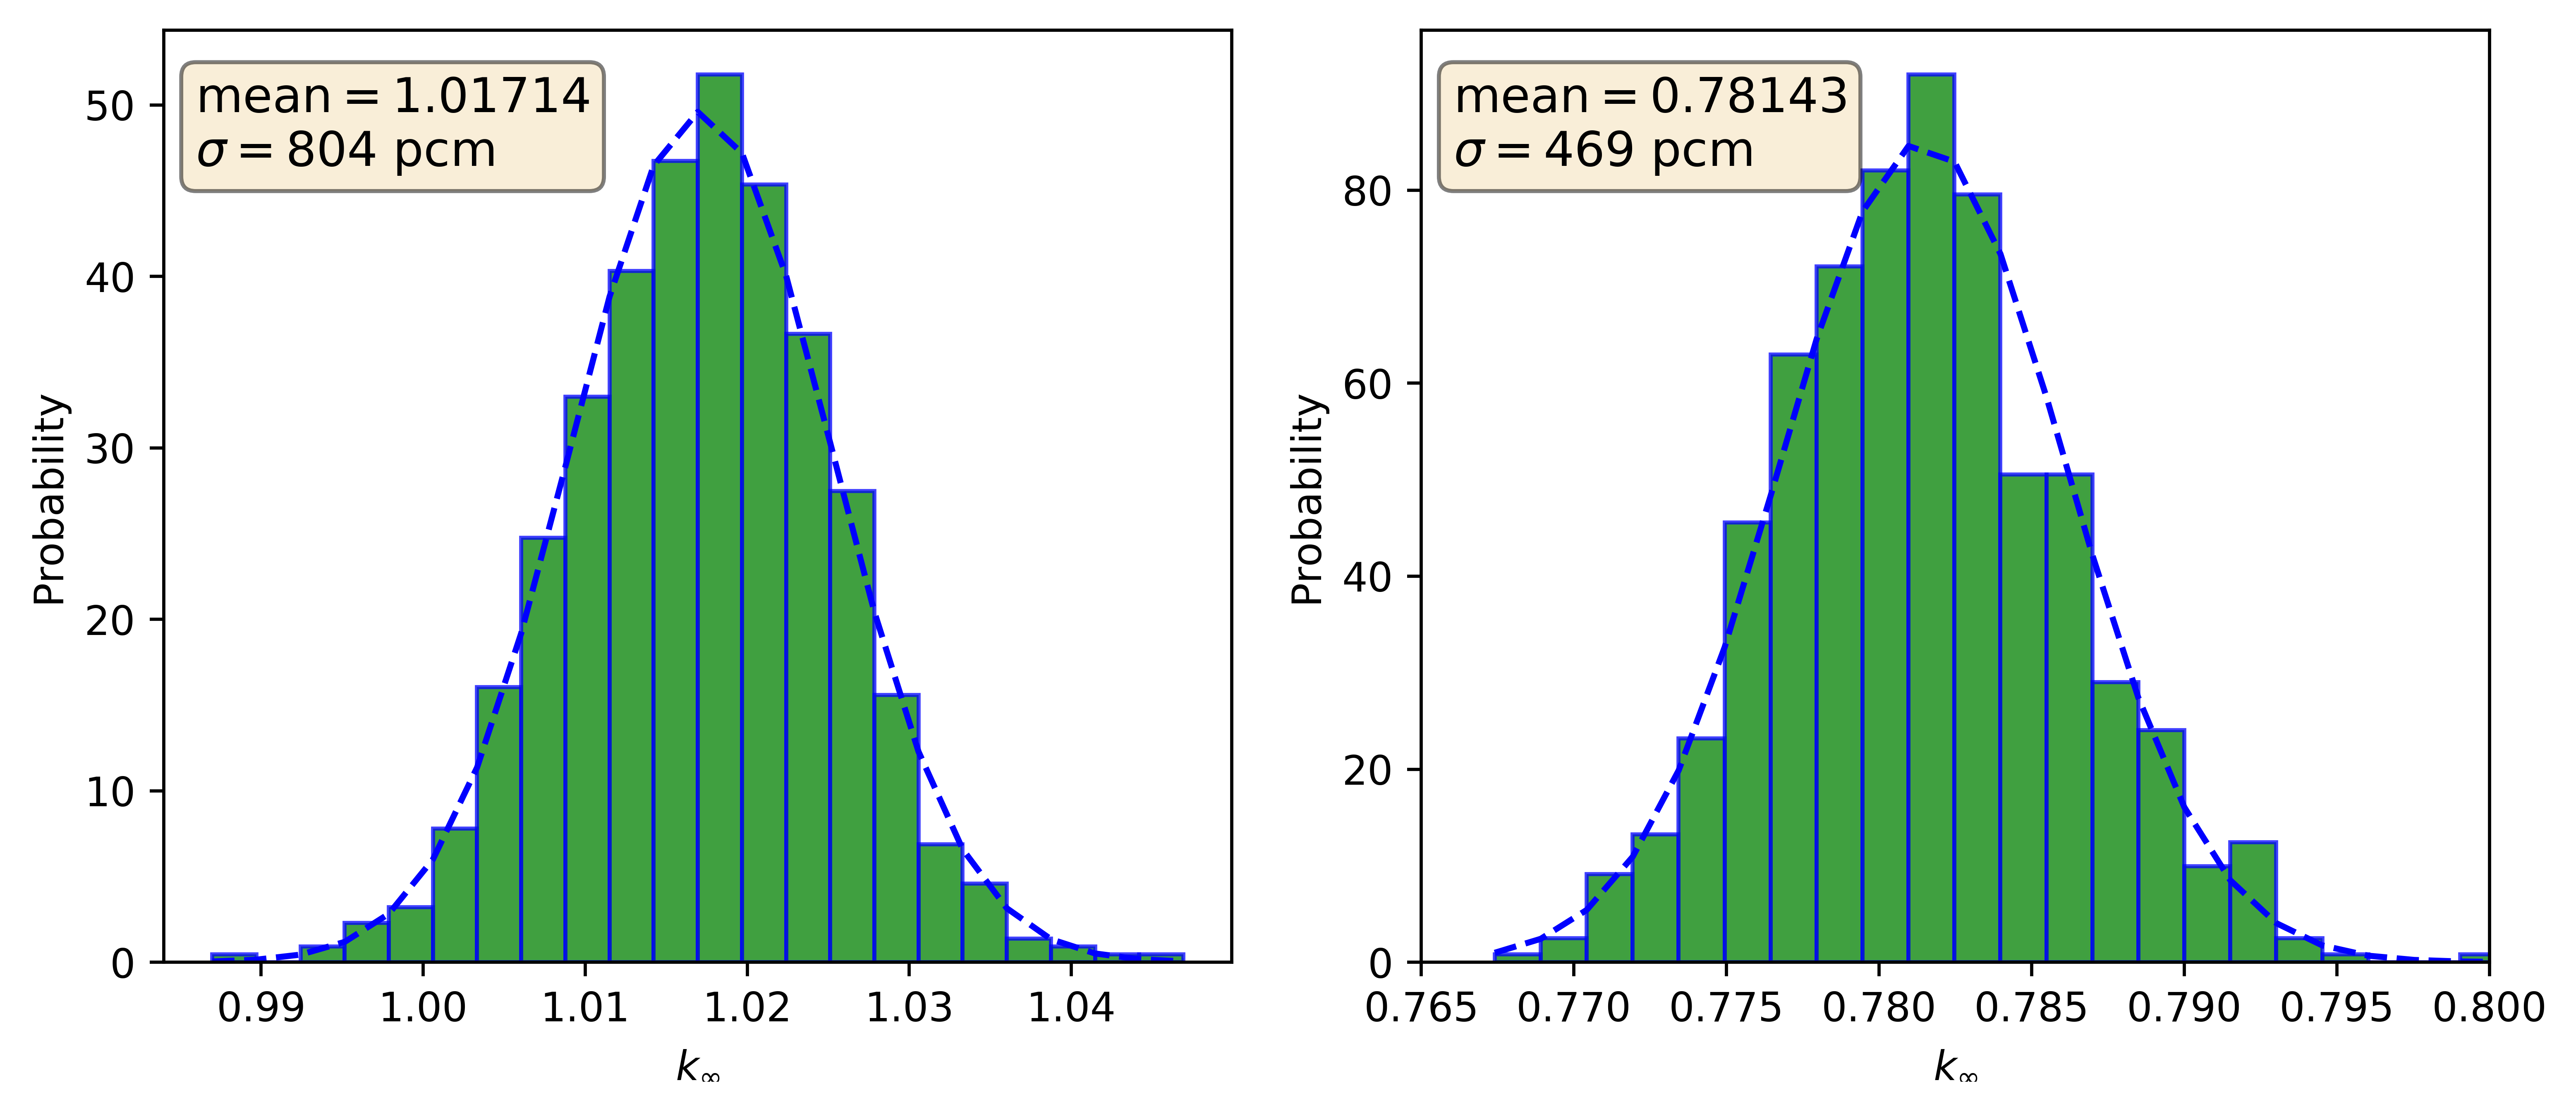
\includegraphics[width=\textwidth]{uq/endf_scale_keff_hist_for_tap.png}
		\vspace{-8mm}
	\caption{Histograms of $k_{\infty}$ samples at the \gls{BOL} (left) and 
		\gls{EOL} (right) obtained with SCALE Sampler by stochastically 
		sampling the nuclear data (cross sections, fission yields, decay 
		constants).}
	\label{fig:uq-scale-kinf-hist}
\end{figure}
\begin{figure}[hbp!] % replace 't' with 'b' to 
	\centering
	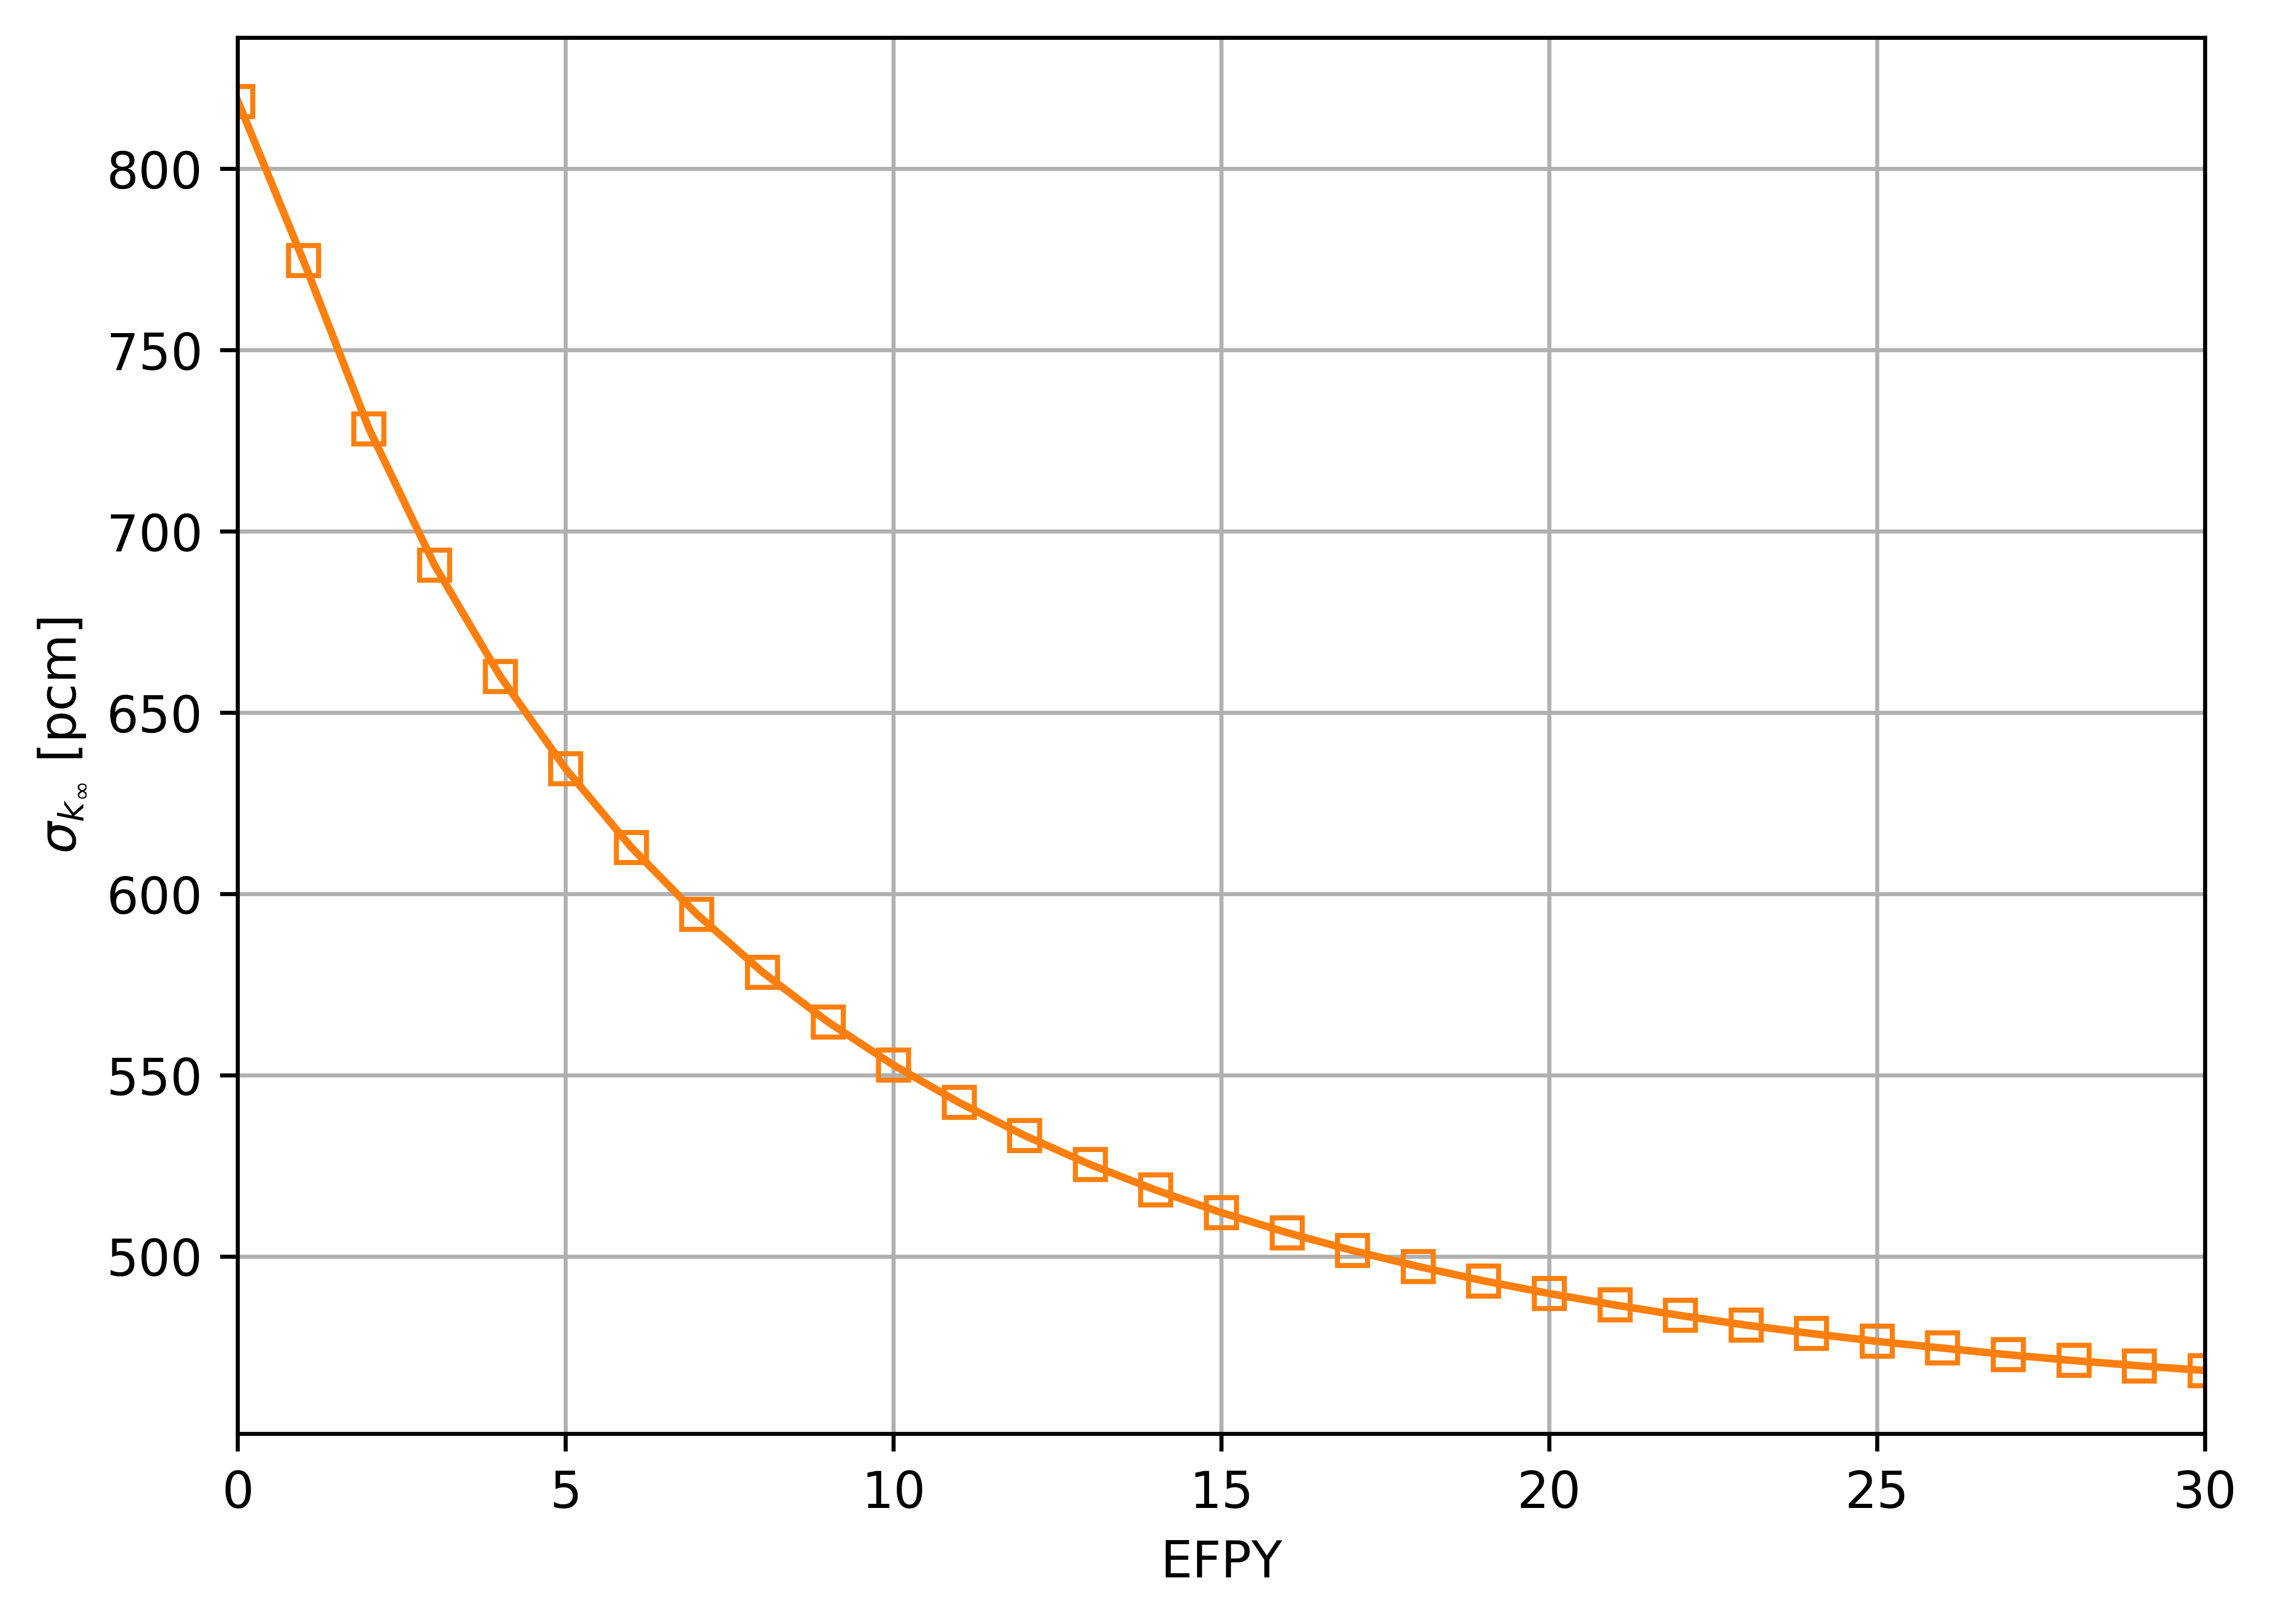
\includegraphics[width=\textwidth]{uq/scale_kinf_dynamics_for_tap.png}
	\caption{Calculated uncertainty in the infinite multiplication factor due 
		to the nuclear data uncertainty as a function of depletion time.}
	\label{fig:uq-scale-kinf}
\end{figure}

Figure~\ref{fig:uq-scale-kinf} demonstrates nuclear data-related uncertainty 
in the $k_{\infty}$ evolution during 30 years of operation. The $k_{\infty}$  
uncertainty decreased slowly because the $k_{\infty}$ mean value reduces over 
time from 1.01714 to 0.78143 due to fuel burnup. Considering more specific 
nuclear data contributions, at the \gls{BOL} the $k_{\infty}$ uncertainty is 
most likely to come from the fissile $^{235}$U fission ($n,f$) and neutron 
capture $(n,\gamma$) reaction cross sections; the $^{238}$U $(n,\gamma$) 
reaction cross section; and the elastic scattering cross section of hydrogen 
in zirconium hydride. However, moving toward the \gls{EOL}, the contributions 
to uncertainty from $^{235}$U data are expected to diminish due to the burnup 
and be substituted by the cross section uncertainties of the fissile plutonium 
(e.g., $^{239}$Pu, $^{241}$Pu). Notably, the $^{235}$U fission cross section 
uncertainty in intermediate and fast spectrum ranges (the \gls{TAP} is an
intermediate spectrum reactor, see Figure~\ref{fig:ben-spectrum-bol}) reaches 
up to 4\%, while it is less than 2.6\% for $^{239}$Pu and $^{241}$Pu. 
$^{239}$Pu and $^{241}$Pu capture and fission cross sections formed the 
dominant source of uncertainty after $^{235}$U was mostly depleted. 
%This $k_{\infty}$ 
%uncertainty evolution is in good agreement with results in the literature  
%\cite{rochman_nuclear_2014, radaideh_advanced_2019}. 

Moreover, the $k_{\infty}$ relative uncertainty from nuclear data slipped 
from 0.78\% at the \gls{BOL} to 0.46\% at the \gls{EOL}. This error is 
slightly larger than results in the literature for conventional \glspl{LWR} 
(e.g., 0.44\% \cite{williams_statistical_2013} or 0.55\% 
\cite{campolina_uncertainty_2018} for a \gls{PWR}). This discrepancy between 
$k_{\infty}$ uncertainty for the \gls{TAP} \gls{MSR} and \gls{PWR} is likely 
to come from $^{19}$F and $^{7}$Li nuclear data, which have significant 
covariances across reactions.

Figure~\ref{fig:uq-scale-u-pu} shows the standard deviation percentages in 
uranium and plutonium isotopic inventory as a function of time. The 
uncertainty in 
$^{238}$U is minimal ($<0.1$\%) and almost constant with burnup because 
$^{238}$U mass does not change significantly from its initial inventory. The 
$^{236}$U uncertainty also is nearly constant during 30 years of operation and 
has a value of $\approx3.8$\%. However, $^{235}$U mass uncertainty increases 
steadily with burnup, due to its inventory decrease during 30 years of 
operation. 
The actual mass uncertainty for $^{235}$U demonstrated growth from 5 kg at 1 
year after startup to approximately 30 kg at the \gls{EOL}.

The uncertainty of major plutonium isotopes (e.g., $^{239}$Pu, $^{240}$Pu, 
$^{241}$Pu) is below 2\% over 30 years of burnup 
(Figure~\ref{fig:uq-scale-u-pu}, lower plot). The fissile $^{239}$Pu and 
poisonous $^{240}$Pu relative standard deviations are increased slightly from 
1.25\% to 1.6\% and from 1.65\% to 1.95\%, respectively. The relative standard 
deviation in fissile $^{241}$Pu mass is significant at the beginning of the 
operation, when its inventory is small (4 kg), and then decreases and 
approaches an equilibrium value of $\approx1.45$\% at the \gls{EOL}. The 
most significant relative standard deviation is observed for $^{242}$Pu mass 
($8.13$\%) because its concentration in fuel is minimal throughout 30 years 
of operation (Table~\ref{tab:uq-scale-mean-std-rsd}).
\begin{figure}[hbp!] % replace 't' with 'b' to 
	\centering
	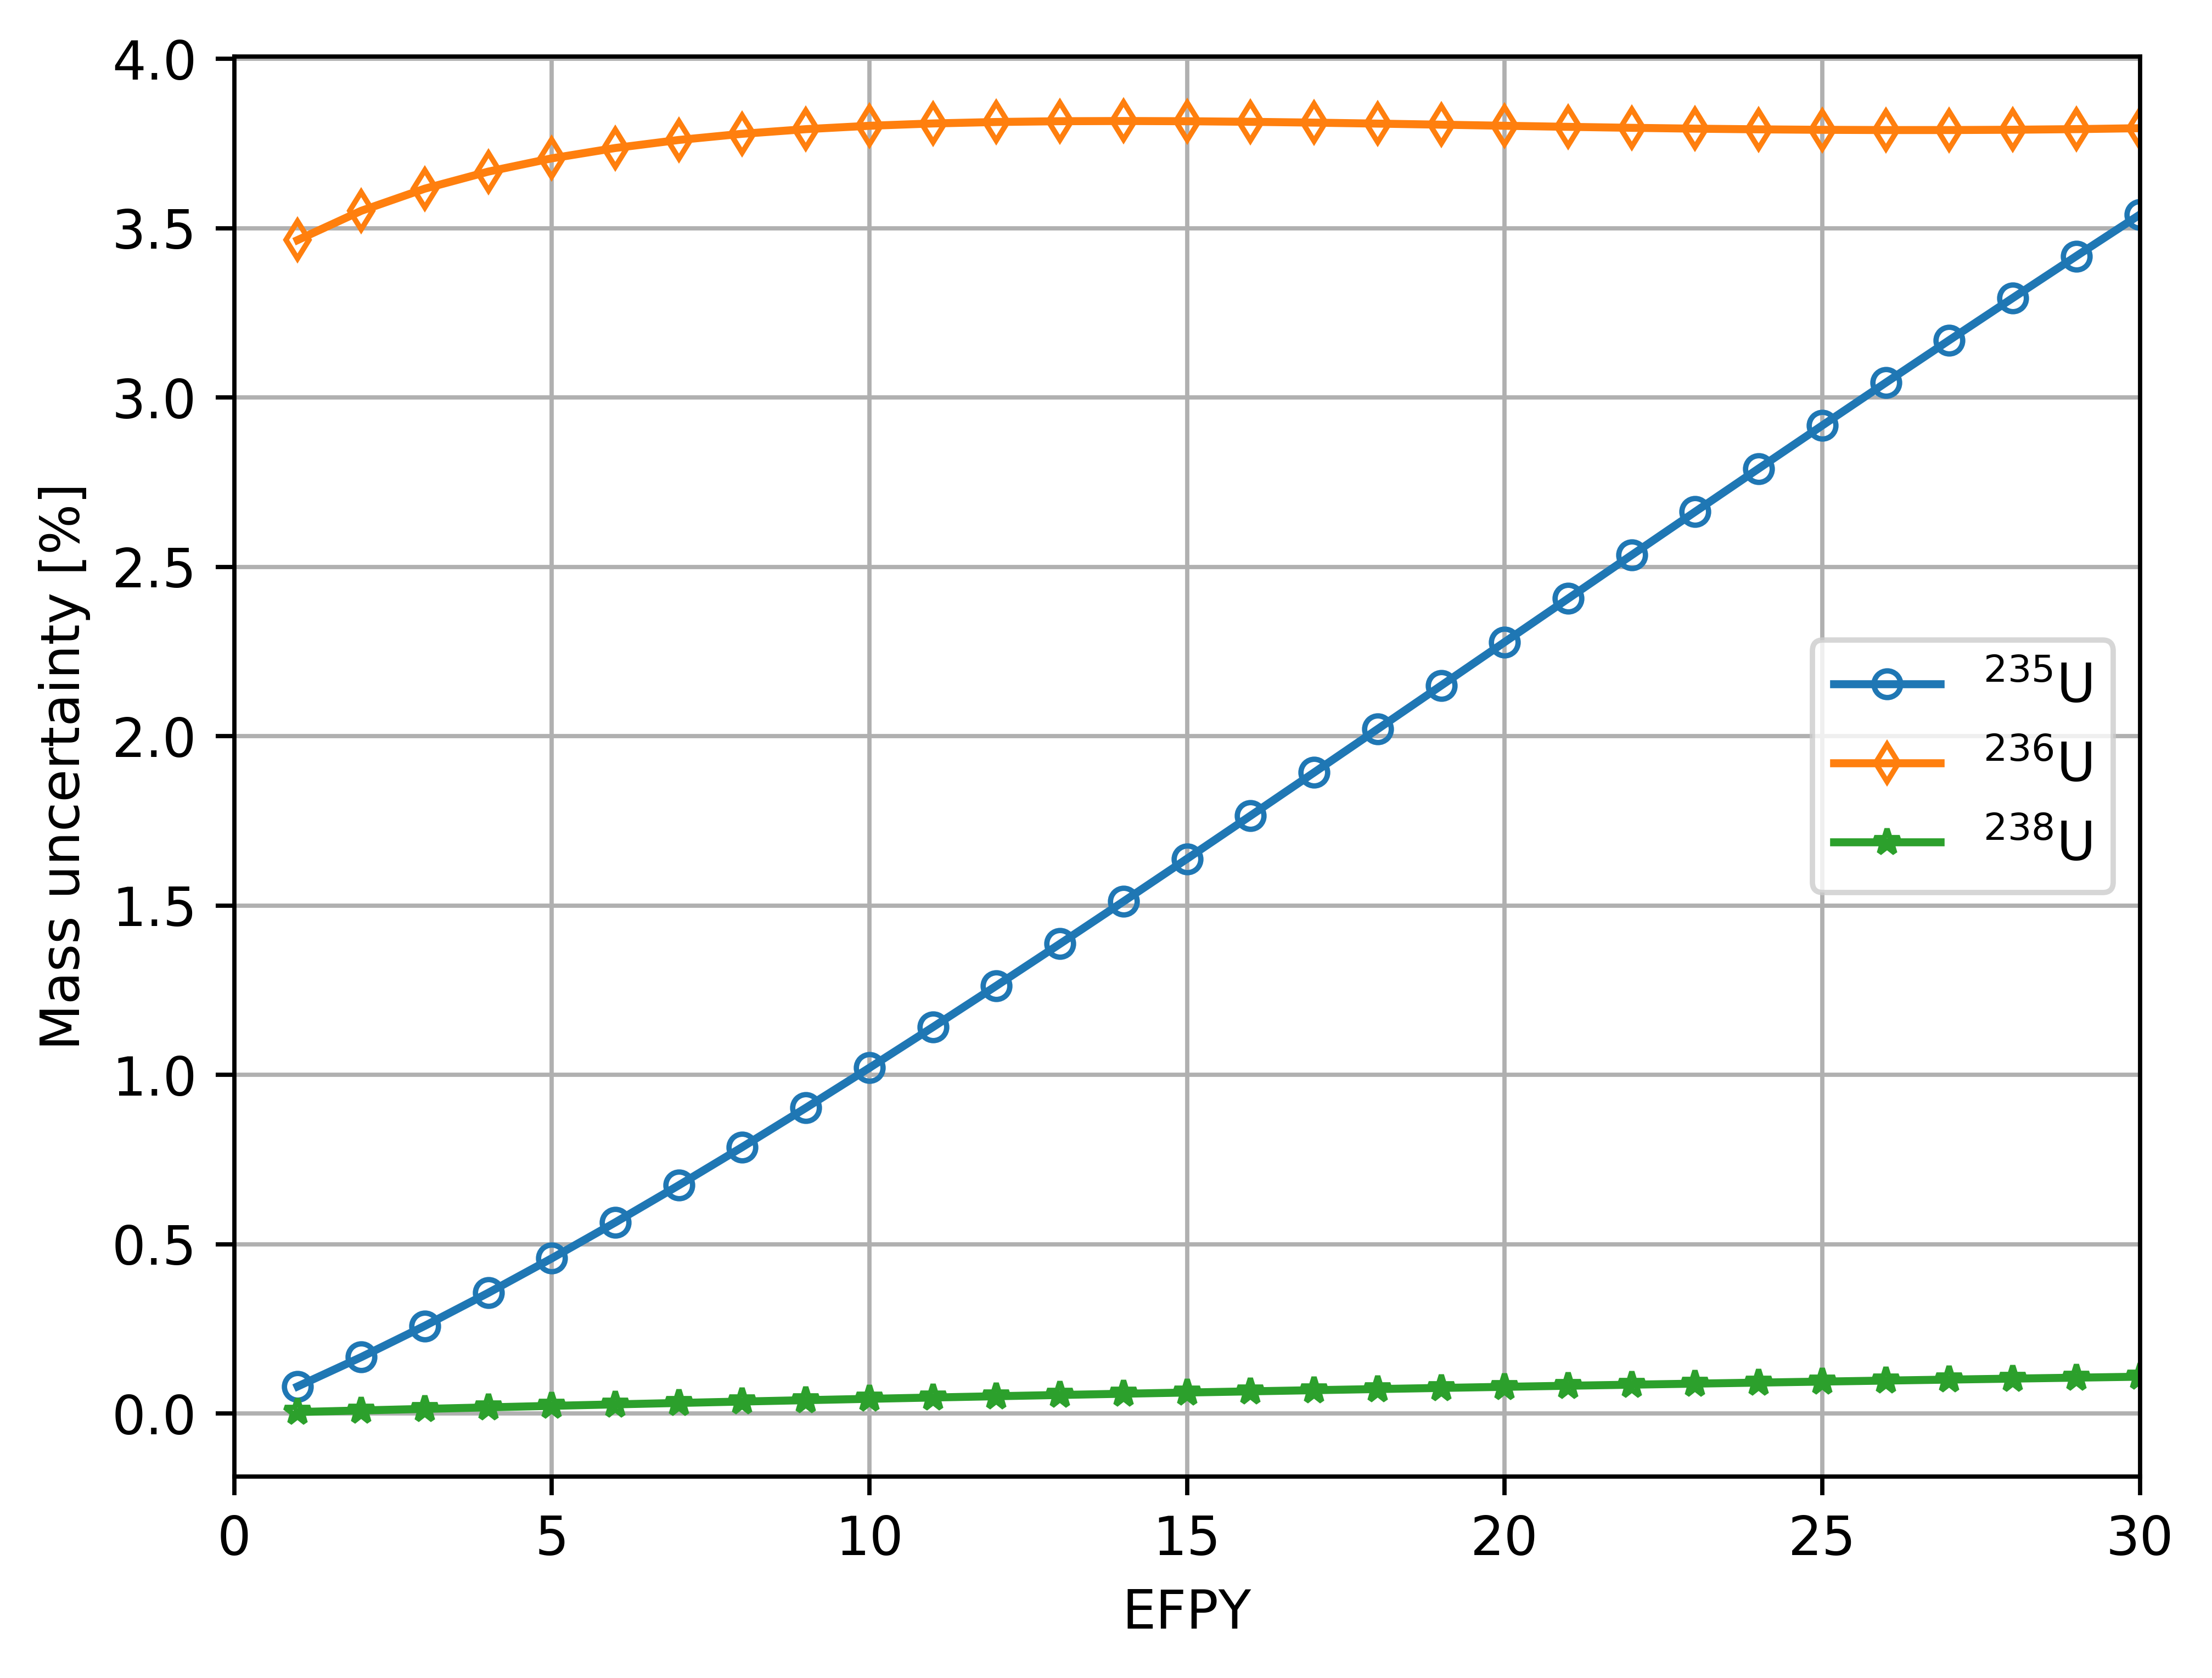
\includegraphics[width=0.85\textwidth]{uq/scale_mass_std_u.png}
		\vspace{-12mm}
	\hspace{0.0mm}
	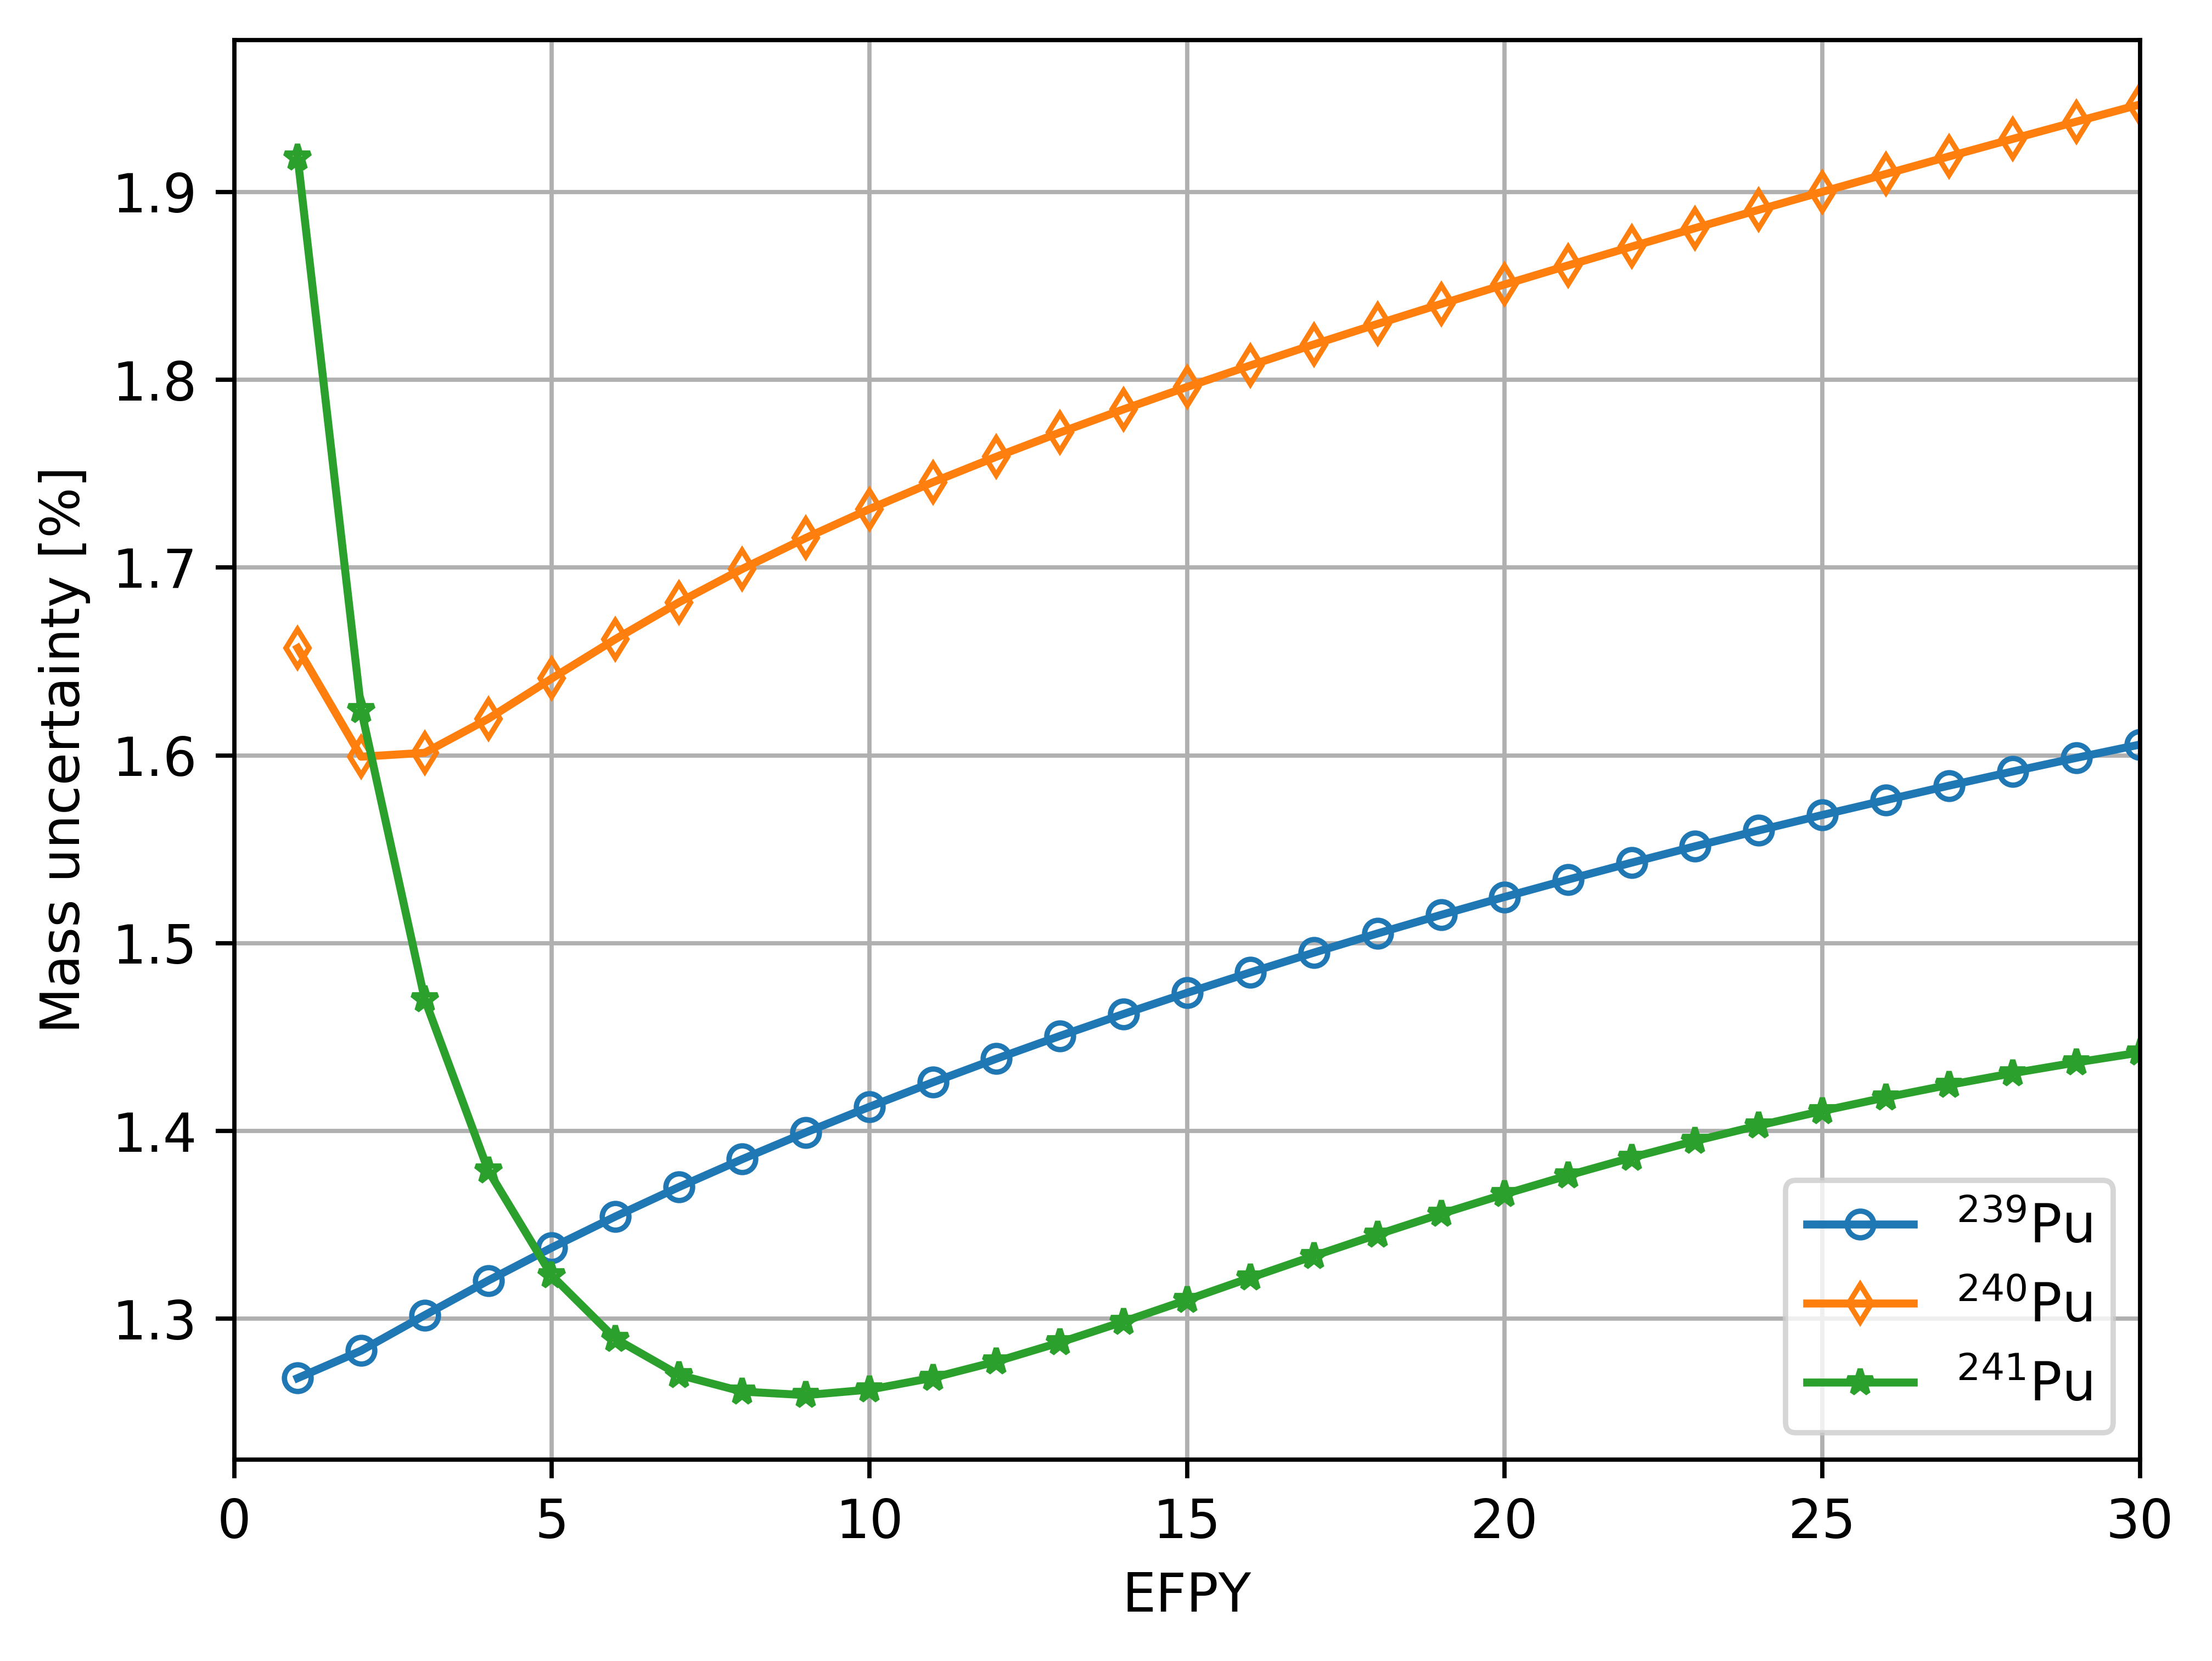
\includegraphics[width=0.85\textwidth]{uq/scale_mass_std_pu.png}
		\vspace{+8mm}
	\caption{Nuclear data-related uncertainty evolution in the uranium (upper) 
	and plutonium (lower) isotopic inventory during 30 years of depletion.}
	\label{fig:uq-scale-u-pu}
\end{figure}

Figure~\ref{fig:uq-scale-xe-i} shows the mass uncertainties for the selected 
\glspl{FP}: $^{135}$Xe and its primary direct precursor, $^{135}$I. The masses 
of $^{135}$Xe and $^{135}$I are in the ranges of 24-27 g and 18-19 g, 
respectively. As expected, relative standard deviations for these isotopes are 
relatively low due to minimal uncertainty of fission yield for $^{235}$U. The 
relative standard deviation of $^{135}$Xe mass changes in a range from 
0.47\% to 0.6\%, while the $^{135}$I standard deviation ranges from 0.35\% to 
0.56\%.
\begin{figure}[hbp!] % replace 't' with 'b' to 
	\centering
	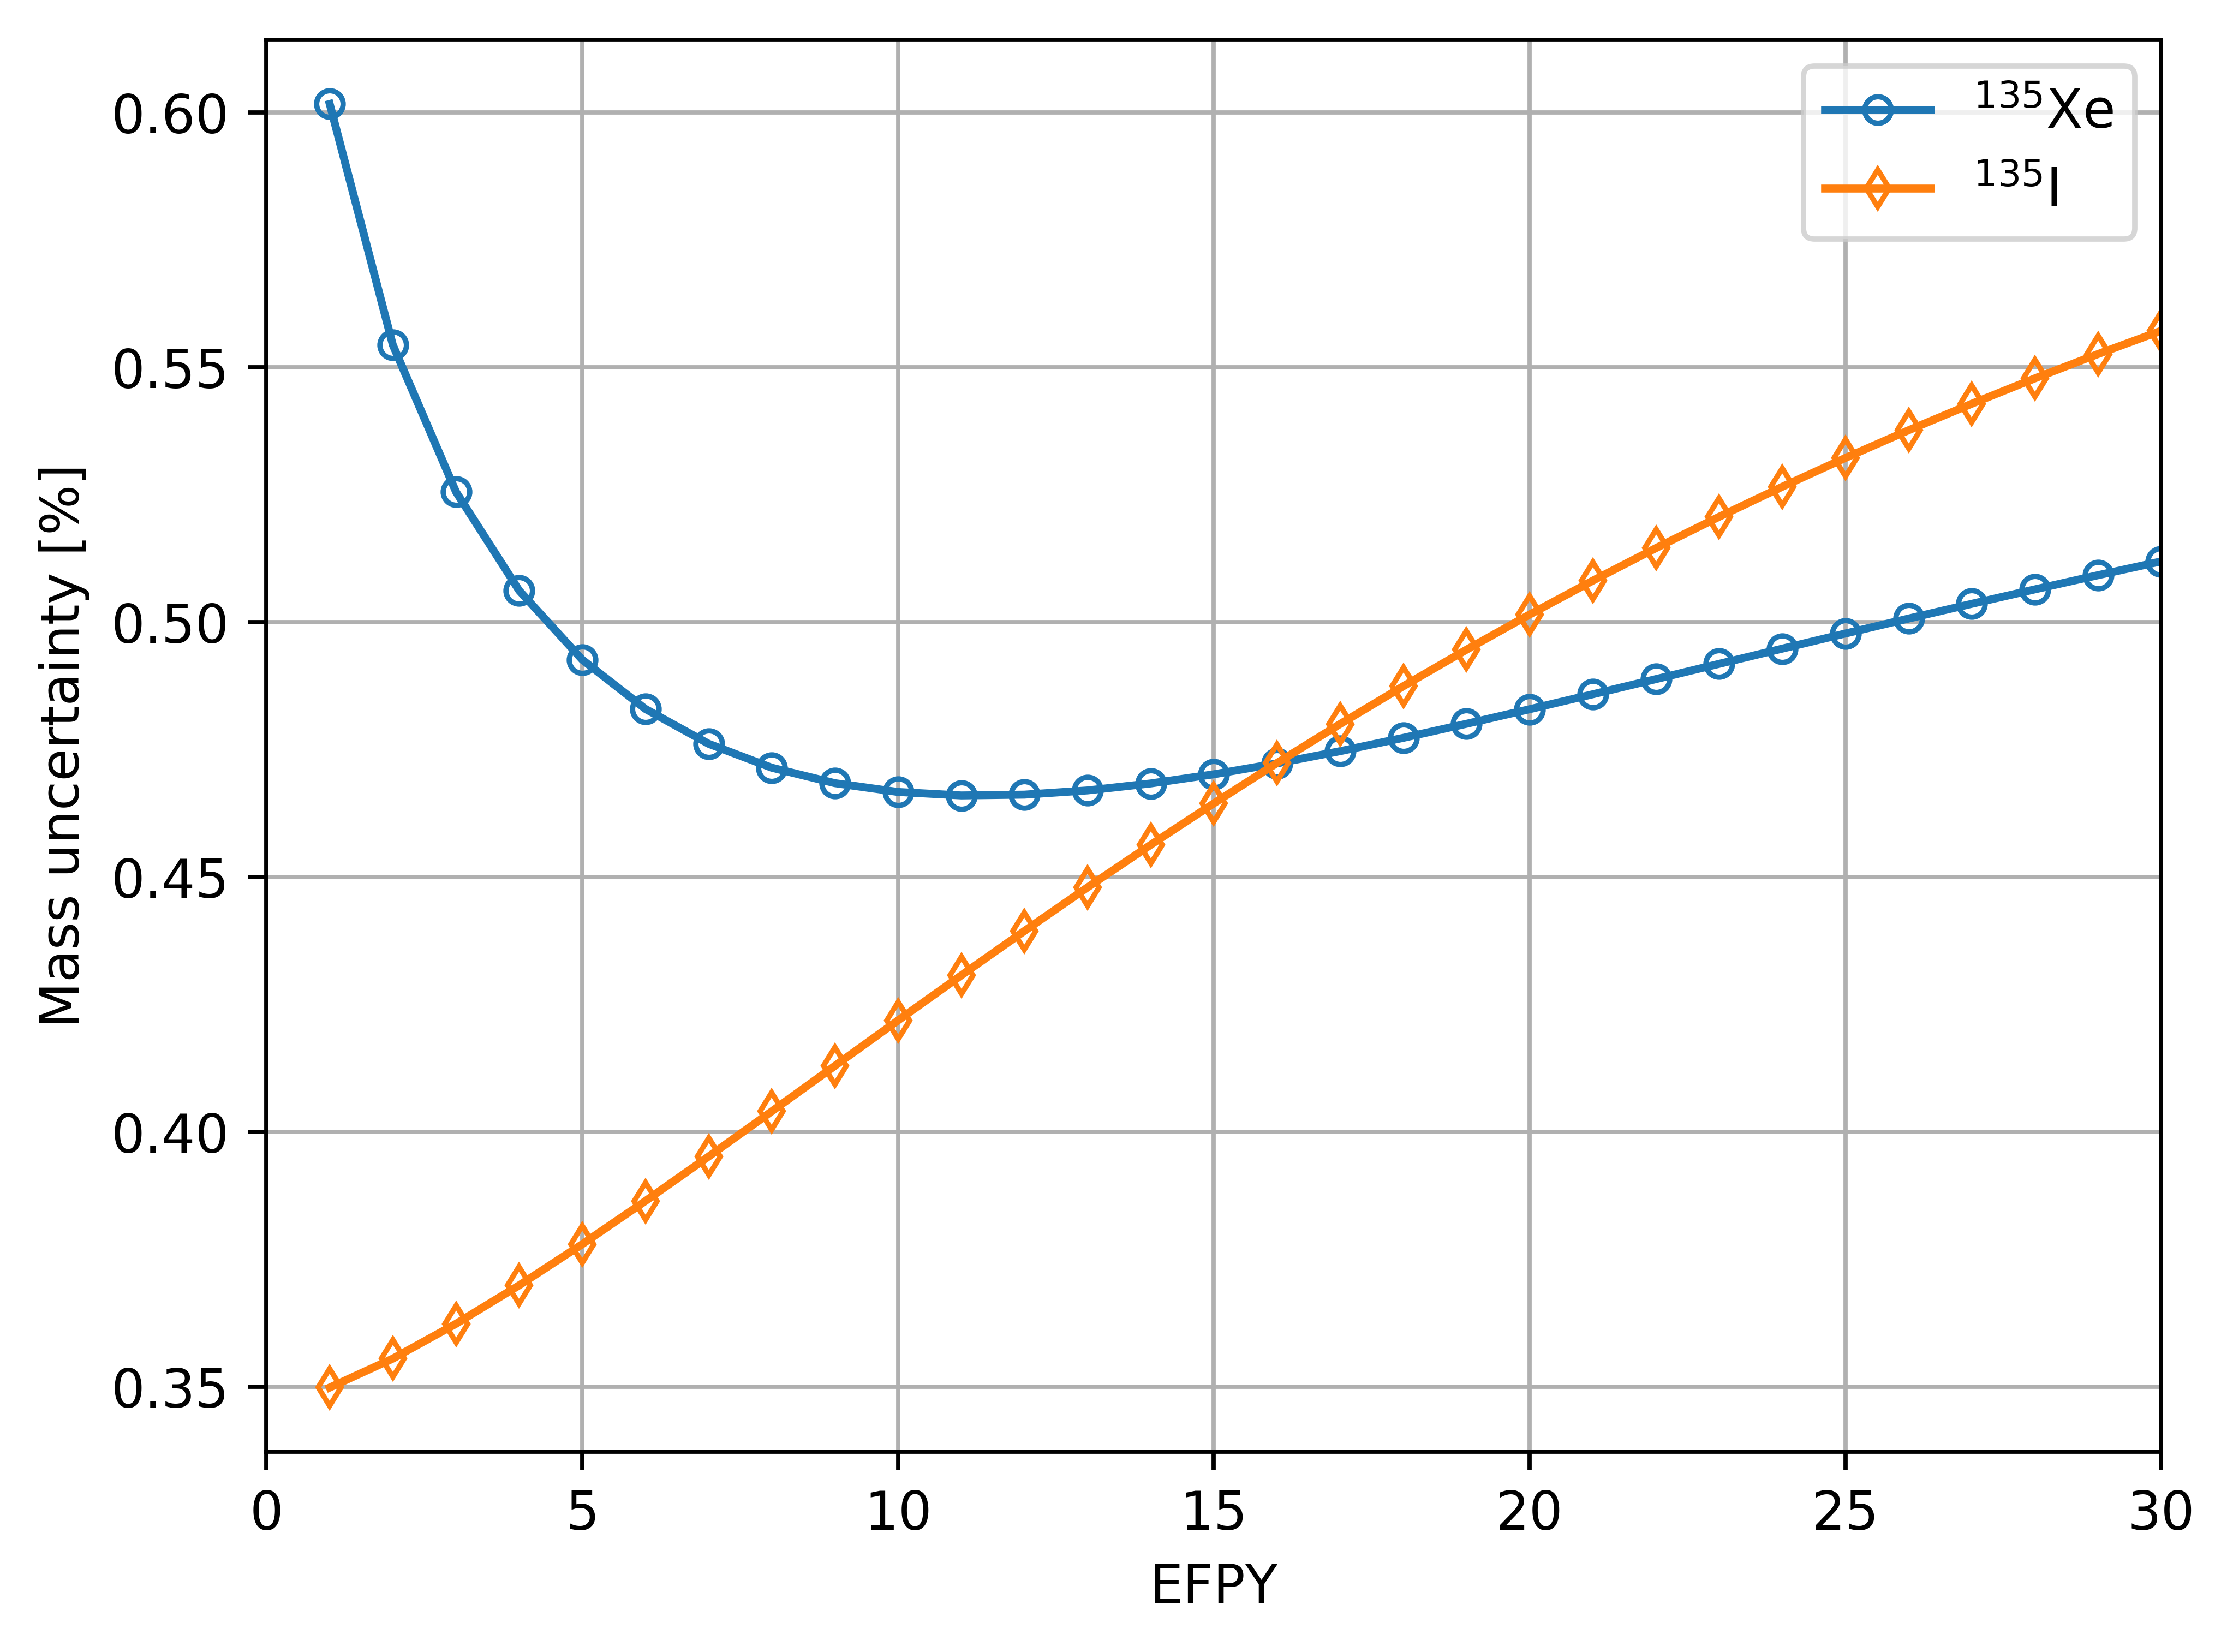
\includegraphics[width=0.85\textwidth]{uq/scale_mass_std_xe_i.png}
	\caption{Nuclear data-related uncertainty evolution in $^{135}$Xe and 
	$^{135}$I isotopic inventory during 30 years of depletion.}
	\label{fig:uq-scale-xe-i}
\end{figure}

Table~\ref{tab:uq-scale-mean-std-rsd} summarizes the nuclear data-related 
uncertainty in the isotopic inventory for the \gls{TAP} \gls{MSR} after 30 
years of operation. Overall, the mass uncertainties due to nuclear data 
uncertainties are two orders of magnitude larger than uncertainty due to 
the statistical error in \gls{MC}.  

All results presented in this section are based on 800 random samples obtained 
using the Sampler tool in SCALE. Figure~\ref{fig:uq-scale-convergence} 
shows the convergence of $k_{\infty}$ and $^{235}$U mass uncertainty with 
number of random samples. Notably, after 500 samples the $k_{\infty}$ and 
$^{235}$U mass uncertainties are stabilized. Overall, 500 random samples is 
enough to accurately estimate uncertainty in the isotopic inventory due to 
uncertainty in nuclear data. 

%%%%%%%%%%%%%%%%%%%%%%%%%%%%%%%%%%%%%%%%
\begin{table}[hbp!]
	\centering
	\caption{Mean value, Standard Deviation (STD), and Relative Standard 
		Deviation (RSD) of mass for the major isotopes after 30-year depletion 
		analysis for the \gls{TAP} reactor. Only nuclear data-related 
		uncertainty is considered.}
	\begin{tabularx}{0.7\textwidth}{L R R R R}
		\hline
		\textbf{Isotope}  & \textbf{Mean [kg]} & \textbf{STD [kg]} & 
		\textbf{RSD [\%]}\\ \hline
		$^{234}$U  & 21.6  & 0.75  & 3.48\% \\
		$^{235}$U  & 839.4 & 29.72 & 3.54\% \\
		$^{236}$U  & 1154.9& 43.83 & 3.79\% \\
		$^{238}$U  & 112,206.1 & 122.32 & 0.11\% \\
		$^{238}$Pu & 335.56& 11.05 & 3.29\% \\
		$^{239}$Pu & 5558.1& 89.25 & 1.61\% \\
		$^{240}$Pu & 1594.6& 31.04 & 1.95\% \\
		$^{241}$Pu & 639.1 & 9.21  & 1.44\% \\
		$^{242}$Pu & 164.0 & 13.33 & 8.13\% \\
		$^{241}$Am & 204.9 & 6.15  & 3.00\% \\
		$^{135}$Xe & 0.03  &$<0.01$& 0.51\% \\
		$^{135}$I  & 0.02  &$<0.01$& 0.56\% \\ \hline
	\end{tabularx}
	\label{tab:uq-scale-mean-std-rsd}
	\vspace{-0.9em}
\end{table}
%%%%%%%%%%%%%%%%%%%%%%%%%%%%%%%%%%%%%%%%%%%%%%%%%%%%%%%%%%%%%%%%%%%%%%%%%%%%%%%


\begin{figure}[hbp!] % replace 't' with 'b' to 
	\centering
	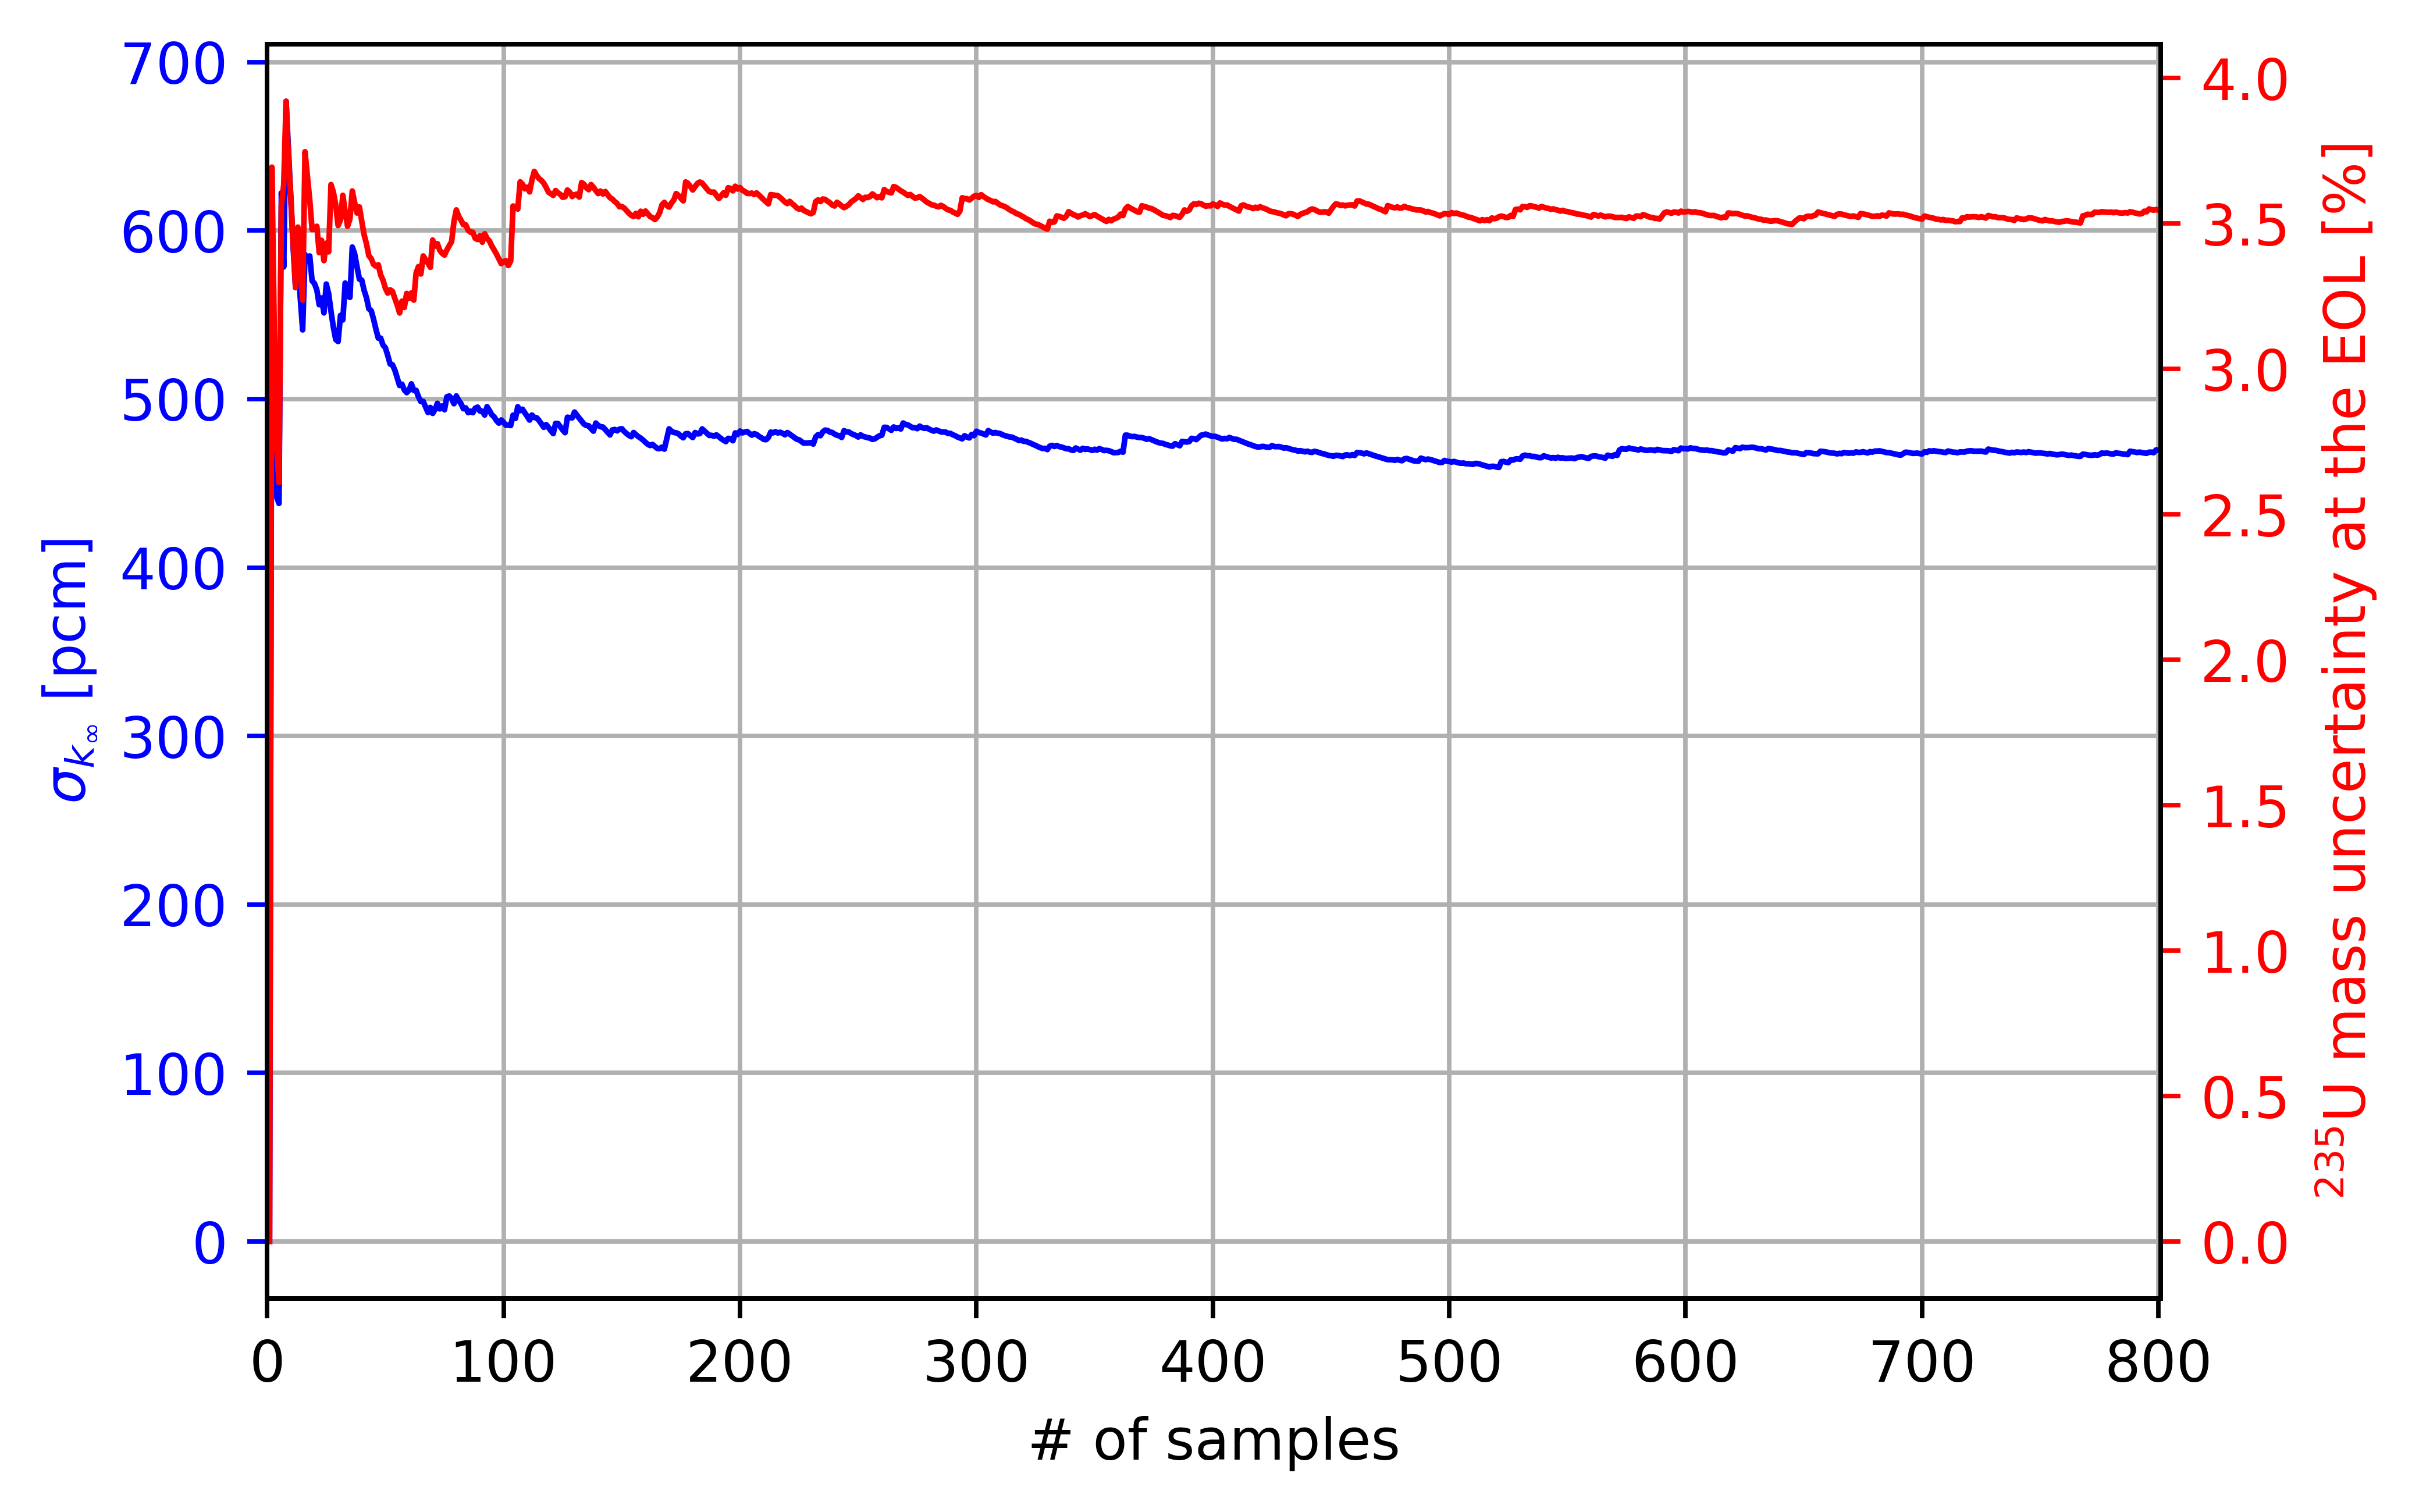
\includegraphics[width=\textwidth]{uq/scale_convergance_for_tap.png}
	\caption{Convergence of $k_{\infty}$ and $^{235}$U mass uncertainties due 
	to the nuclear data uncertainty as a function of the number of samples for 
	simulation using SCALE with the Sampler module.}
	\label{fig:uq-scale-convergence}
\end{figure}

\section{Concluding remarks}
Uncertainty propagation analysis was performed for the depletion calculation 
for the \gls{TAP} \gls{MSR} 30-year burnup. I separately considered two 
primary sources of uncertainty in the depletion calculations: stochastic 
uncertainty in the neutron flux distribution and uncertainty in the nuclear 
data. Stochastic error in the isotopic composition was obtained using the 
Serpent Continuous Energy Monte Carlo code by running the same depletion 
sequence 1000 times, each time with a new unique initial seed number. The 
Sampler module in SCALE 6.2 with a 56-group covariance library was used to 
obtain nuclear data-related uncertainty in the isotopic composition of the 
fuel salt. 
Uncertainties in the input nuclear data (cross sections, fission yields, decay 
constants) are propagated throughout all steps of the transport/depletion 
sequence, including self-shielding, space-energy flux calculation, and isotope 
transmutation. 

The errors in isotopic masses due to the statistical errors are below 0.067\% 
for 7.5 million neutron histories (total neutron flux relative stochastic 
error $<0.01$\%). Therefore, it is unnecessary to consider the accumulation of 
the stochastic error for the fuel depletion in the \gls{TAP} reactor 
considered in this dissertation.
Finally, the stochastic error in the isotopic inventory could be reduced to 
almost zero by increasing the number of neutron histories, but it is 
impractical due to the sublinear convergence rate of the Monte Carlo method 
($O(\sqrt{N})$).

On the other hand, the computed errors in the isotopic inventory due to the 
nuclear data uncertainties are a few orders of magnitude larger and cannot 
be ignored. The nuclear data-related errors are in the range from 1\% to 2\% 
for the masses of $^{239}$Pu, $^{240}$Pu, and $^{241}$Pu, and about 3-8\% for  
$^{234}$U,$^{235}$U, $^{236}$U, $^{238}$Pu, $^{242}$Pu, and $^{241}$Am. 
Finally, the mass uncertainty for the selected \glspl{FP} ($^{135}$Xe and 
$^{135}$I), which are the subject of interest of the current work, is below 
0.6\%. Overall, the principal source of uncertainty in depletion calculations 
is related to the nuclear data covariances.

Finally, this chapter demonstrated that the standard deviation in the 
multiplication factor due to the nuclear data uncertainty ranges from 804 to 
469 $pcm$, while the stochastic error is only about 30 $pcm$. Overall, to 
accurately capture the isotopic inventory evolution for the \gls{TAP} concept 
using SaltProc v1.0 with Serpent Monte Carlo code, it is unnecessary to 
waste a vast computational power to simulate $10^7-10^9$ neutron histories per 
each depletion step because the impact of the stochastic errors in 
neutron fluxes is negligible compared with the nuclear data-related errors .